% Options for packages loaded elsewhere
\PassOptionsToPackage{unicode}{hyperref}
\PassOptionsToPackage{hyphens}{url}
%
\documentclass[
]{article}
\usepackage{amsmath,amssymb}
\usepackage{lmodern}
\usepackage{iftex}
\ifPDFTeX
  \usepackage[T1]{fontenc}
  \usepackage[utf8]{inputenc}
  \usepackage{textcomp} % provide euro and other symbols
\else % if luatex or xetex
  \usepackage{unicode-math}
  \defaultfontfeatures{Scale=MatchLowercase}
  \defaultfontfeatures[\rmfamily]{Ligatures=TeX,Scale=1}
\fi
% Use upquote if available, for straight quotes in verbatim environments
\IfFileExists{upquote.sty}{\usepackage{upquote}}{}
\IfFileExists{microtype.sty}{% use microtype if available
  \usepackage[]{microtype}
  \UseMicrotypeSet[protrusion]{basicmath} % disable protrusion for tt fonts
}{}
\makeatletter
\@ifundefined{KOMAClassName}{% if non-KOMA class
  \IfFileExists{parskip.sty}{%
    \usepackage{parskip}
  }{% else
    \setlength{\parindent}{0pt}
    \setlength{\parskip}{6pt plus 2pt minus 1pt}}
}{% if KOMA class
  \KOMAoptions{parskip=half}}
\makeatother
\usepackage{xcolor}
\usepackage[margin=1in]{geometry}
\usepackage{color}
\usepackage{fancyvrb}
\newcommand{\VerbBar}{|}
\newcommand{\VERB}{\Verb[commandchars=\\\{\}]}
\DefineVerbatimEnvironment{Highlighting}{Verbatim}{commandchars=\\\{\}}
% Add ',fontsize=\small' for more characters per line
\usepackage{framed}
\definecolor{shadecolor}{RGB}{248,248,248}
\newenvironment{Shaded}{\begin{snugshade}}{\end{snugshade}}
\newcommand{\AlertTok}[1]{\textcolor[rgb]{0.94,0.16,0.16}{#1}}
\newcommand{\AnnotationTok}[1]{\textcolor[rgb]{0.56,0.35,0.01}{\textbf{\textit{#1}}}}
\newcommand{\AttributeTok}[1]{\textcolor[rgb]{0.77,0.63,0.00}{#1}}
\newcommand{\BaseNTok}[1]{\textcolor[rgb]{0.00,0.00,0.81}{#1}}
\newcommand{\BuiltInTok}[1]{#1}
\newcommand{\CharTok}[1]{\textcolor[rgb]{0.31,0.60,0.02}{#1}}
\newcommand{\CommentTok}[1]{\textcolor[rgb]{0.56,0.35,0.01}{\textit{#1}}}
\newcommand{\CommentVarTok}[1]{\textcolor[rgb]{0.56,0.35,0.01}{\textbf{\textit{#1}}}}
\newcommand{\ConstantTok}[1]{\textcolor[rgb]{0.00,0.00,0.00}{#1}}
\newcommand{\ControlFlowTok}[1]{\textcolor[rgb]{0.13,0.29,0.53}{\textbf{#1}}}
\newcommand{\DataTypeTok}[1]{\textcolor[rgb]{0.13,0.29,0.53}{#1}}
\newcommand{\DecValTok}[1]{\textcolor[rgb]{0.00,0.00,0.81}{#1}}
\newcommand{\DocumentationTok}[1]{\textcolor[rgb]{0.56,0.35,0.01}{\textbf{\textit{#1}}}}
\newcommand{\ErrorTok}[1]{\textcolor[rgb]{0.64,0.00,0.00}{\textbf{#1}}}
\newcommand{\ExtensionTok}[1]{#1}
\newcommand{\FloatTok}[1]{\textcolor[rgb]{0.00,0.00,0.81}{#1}}
\newcommand{\FunctionTok}[1]{\textcolor[rgb]{0.00,0.00,0.00}{#1}}
\newcommand{\ImportTok}[1]{#1}
\newcommand{\InformationTok}[1]{\textcolor[rgb]{0.56,0.35,0.01}{\textbf{\textit{#1}}}}
\newcommand{\KeywordTok}[1]{\textcolor[rgb]{0.13,0.29,0.53}{\textbf{#1}}}
\newcommand{\NormalTok}[1]{#1}
\newcommand{\OperatorTok}[1]{\textcolor[rgb]{0.81,0.36,0.00}{\textbf{#1}}}
\newcommand{\OtherTok}[1]{\textcolor[rgb]{0.56,0.35,0.01}{#1}}
\newcommand{\PreprocessorTok}[1]{\textcolor[rgb]{0.56,0.35,0.01}{\textit{#1}}}
\newcommand{\RegionMarkerTok}[1]{#1}
\newcommand{\SpecialCharTok}[1]{\textcolor[rgb]{0.00,0.00,0.00}{#1}}
\newcommand{\SpecialStringTok}[1]{\textcolor[rgb]{0.31,0.60,0.02}{#1}}
\newcommand{\StringTok}[1]{\textcolor[rgb]{0.31,0.60,0.02}{#1}}
\newcommand{\VariableTok}[1]{\textcolor[rgb]{0.00,0.00,0.00}{#1}}
\newcommand{\VerbatimStringTok}[1]{\textcolor[rgb]{0.31,0.60,0.02}{#1}}
\newcommand{\WarningTok}[1]{\textcolor[rgb]{0.56,0.35,0.01}{\textbf{\textit{#1}}}}
\usepackage{graphicx}
\makeatletter
\def\maxwidth{\ifdim\Gin@nat@width>\linewidth\linewidth\else\Gin@nat@width\fi}
\def\maxheight{\ifdim\Gin@nat@height>\textheight\textheight\else\Gin@nat@height\fi}
\makeatother
% Scale images if necessary, so that they will not overflow the page
% margins by default, and it is still possible to overwrite the defaults
% using explicit options in \includegraphics[width, height, ...]{}
\setkeys{Gin}{width=\maxwidth,height=\maxheight,keepaspectratio}
% Set default figure placement to htbp
\makeatletter
\def\fps@figure{htbp}
\makeatother
\setlength{\emergencystretch}{3em} % prevent overfull lines
\providecommand{\tightlist}{%
  \setlength{\itemsep}{0pt}\setlength{\parskip}{0pt}}
\setcounter{secnumdepth}{-\maxdimen} % remove section numbering
\ifLuaTeX
  \usepackage{selnolig}  % disable illegal ligatures
\fi
\IfFileExists{bookmark.sty}{\usepackage{bookmark}}{\usepackage{hyperref}}
\IfFileExists{xurl.sty}{\usepackage{xurl}}{} % add URL line breaks if available
\urlstyle{same} % disable monospaced font for URLs
\hypersetup{
  pdftitle={Stats 15 Project},
  pdfauthor={Team 13: Wanyue Dong, Michelle Pang, Liaohan Wang},
  hidelinks,
  pdfcreator={LaTeX via pandoc}}

\title{Stats 15 Project}
\author{Team 13: Wanyue Dong, Michelle Pang, Liaohan Wang}
\date{10/31/2022}

\begin{document}
\maketitle

\hypertarget{section-1---introduction}{%
\section{\texorpdfstring{\textbf{Section 1 -
Introduction}}{Section 1 - Introduction}}\label{section-1---introduction}}

\hypertarget{motivating-questions-and-scope-of-analysis}{%
\subsection{\texorpdfstring{\textbf{1.1 - Motivating Questions and Scope
of
Analysis}}{1.1 - Motivating Questions and Scope of Analysis}}\label{motivating-questions-and-scope-of-analysis}}

As one of the biggest cities in China, Beijing currently houses a
population of 21.33 million residents. With the rapid rate of
globalization, the movement of people selling and buying their property
has risen as well. However, with the help of Lianjia, buyers and sellers
are able to view and list properties with ease. In this project, we seek
to answer the following motivating question: \textbf{what affects the
price per square foot of a property?}

\hypertarget{background-on-lianjia}{%
\subsection{\texorpdfstring{\textbf{1.2 - Background on
Lianjia}}{1.2 - Background on Lianjia}}\label{background-on-lianjia}}

\textbf{\emph{Basic Structure:}} Lianjia is a Chinese real-estate
company that allows buyers and sellers to view and list properties all
over China on the Lianjia website. In our data set, we narrowed down our
listings to those that were traded in 2017 in the city of Beijing. This
means that any property that was listed or sold in 2017 will be included
and the others will be excluded. We found our data set on a website
called Kaggle which is a data science company which provides a variety
of public data sets. Before cleaning the data, our data set had 318,815
listings and 26 variables.

\textbf{\emph{How a Seller can Post a Listing:}} To post a listing on
Lianjia, the owner or the real estate agent of the property will have to
follow the guidelines and steps provided by filling out the necessary
information regarding the property such as price of listing, number of
bathrooms, square footage of the entire property and more listed below
in the explanatory variables. They will also need to provide
accompanying photographs of the property.

\textbf{\emph{How a Buyer can Purchase a Listing:}} To purchase a
listing on Lianjia, the buyer can simply just reach out to the contact
number or email of the real estate angent provided to arrange a viewing.
After viewing the property and possible negotiations, both parties will
agree on a price for the transaction and legal paperwork will be
organized by the real estate agency to facilitate the payment process
and finally legalize the change of ownership of the property.

\textbf{\emph{Beijing Districts:}} There are a total of 13 districts
within Beijing that we will be focusing on. These 13 districts include
DongCheng, FengTai, YiZhuang, DaXing, FangShan, ChangPing, ChaoYang,
HaiDian, ShiJingShan, XiCheng, TongZhou, MenTouGou and ShunYi. Each
listing in our data set lies in one of these 13 districts.

There are a total of 16 districts in Beijing, but we mainly focuses on
the listed 13 districts which are shown on the map as yellow, red, and
purple. Yellow and red parts are considered the core districts. In other
words, ``the city''. They contains the main functions of Beijing in
political, cultural and economic ways. The yellow parts, DongCheng and
XiCheng contain the most history of the city. They have a relative small
area but most ancient buildings preserved. Thus, there are actually not
that much area could be used for residency nor new structures. Among
these red parts, ChaoYang and HaiDian are a bit special. ChaoYang is the
largest among the core districts. It has the majority of foreign
embassies and it is also the business center. HaiDian is famous for
education. It contains the most education institutions. Purple parts are
considered suburb areas where airports are located. Green parts are
excluded from our data because these are relative rural that are mostly
made up of mountains, Great Walls, manors for travelers, etc.

\hypertarget{variable-explanation}{%
\subsection{\texorpdfstring{\textbf{1.3 - Variable
Explanation}}{1.3 - Variable Explanation}}\label{variable-explanation}}

\hypertarget{explanatory-variables}{%
\subsubsection{\texorpdfstring{\textbf{Explanatory
Variables}}{Explanatory Variables}}\label{explanatory-variables}}

\begin{enumerate}
\def\labelenumi{\arabic{enumi}.}
\tightlist
\item
  \textbf{\emph{DOM}}: (\emph{numerical}) The active days on market. The
  number of days since the property is posted until it is sold and
  removed from the website.
\item
  \textbf{\emph{followers}}: (\emph{numerical}) The number of people who
  follow the transaction by bookmarking the property to revisit later
  on. This indicates the popularity of a property compared to the other
  listings.
\item
  \textbf{\emph{livingRoom}}: (\emph{numerical}) The number of bedrooms.
\item
  \textbf{\emph{drawingRoom}}: (\emph{numerical}) The number of living
  rooms.
\item
  \textbf{\emph{kitchen}}: (\emph{numerical}) The number of kitchens.
\item
  \textbf{\emph{bathRoom}}: (\emph{numerical}) The number of bathrooms.
\item
  \textbf{\emph{floor}}: (\emph{numerical}) The total number of floors
  the building has. This usually also refers to the height of the
  building.
\item
  \textbf{\emph{constructionTime}}: (\emph{categorical}) The year the
  building was constructed.
\item
  \textbf{\emph{renovationCondition}}: (\emph{categorical}) The quality
  of the renovation with 4 being the best and 1 being the worst.
\item
  \textbf{\emph{buildingStructure}}: (\emph{categorical}) The material
  that is used the most to construct the building. More specifically,
  the main material used to build the exterior of the building. In this
  case, 1 refers to the material being unknown, 2 refers to the material
  being a mix of more than 3 distinguishable materials, 3 refers to
  brick and wood, 4 refers to brick and concrete, 5 refers to steel and
  6 refers to steel-concrete composite.
\item
  \textbf{\emph{ladderRatio}}: (\emph{categorical}) The proportion
  between number of residents who live on the same floor to the number
  of elevators or ladders that particular floor has. It relates to the
  frequency of usage of the elevator per floor. In this case, 1.00
  refers to the highest frequency of usage and 0.00 refers to lowest
  frequency of usage.
\item
  \textbf{\emph{elevator}}: (\emph{categorical}) The presence of an
  elevator or not. In this case, 1 refers to the presence of an elevator
  in the building and 0 refers to the absence of an elevator in the
  building.
\item
  \textbf{\emph{fiveYearsProperty}}: (\emph{categorical}) Refers to
  whether or not the previous owner has owned the property for less than
  five years. In this case, 1 refers to the property being owned by the
  previous owner for less than five years and 0 refers to the property
  being owned by the previous owner for more than five years.
\item
  \textbf{\emph{subway}}: (\emph{categorical}) Based on the knowledge of
  the seller posting the listing, this variable shows if a subway is
  located near the property. In this case, 1 refers to the presence of a
  subway nearby and 0 refers to the absence of a subway nearby.
\end{enumerate}

\begin{figure}
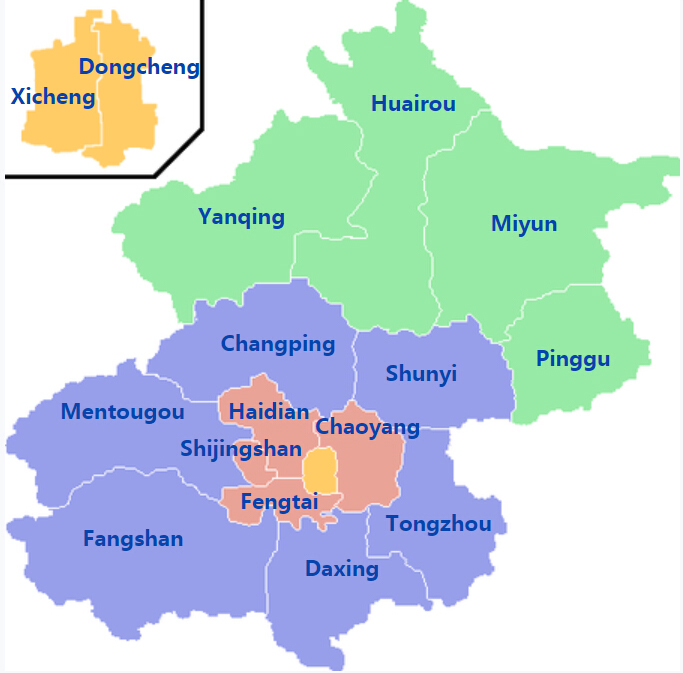
\includegraphics[width=0.5\linewidth]{beijing_map} \caption{Beijing District Map}\label{fig:pressure}
\end{figure}

\begin{enumerate}
\def\labelenumi{\arabic{enumi}.}
\setcounter{enumi}{14}
\tightlist
\item
  \textbf{\emph{district}}: (\emph{categorical}) There are 13 main
  districts in Beijing and each number from 1 to 13 refers to a
  different district in which the property lies in. In this case, 1
  refers to DongCheng, 2 refers to FengTai, 3 refers to YiZhuang, 4
  refers to DaXing, 5 refers to FangShan, 6 refers to ChangPing, 7
  refers to ChaoYang, 8 refers to HaiDian, 9 refers to ShiJingShan, 10
  refers to XiCheng, 11 refers to TongZhou, 12 refers to MenTouGou and
  13 refers to ShunYi.
\end{enumerate}

\hypertarget{response-variable}{%
\subsubsection{\texorpdfstring{\textbf{Response
Variable}}{Response Variable}}\label{response-variable}}

\begin{enumerate}
\def\labelenumi{\arabic{enumi}.}
\tightlist
\item
  \textbf{\emph{price}}: (\emph{integer}) The price per square foot of
  the property (price = totalPrice / square). To ensure that the price
  is a fair comparison across all the properties listed, we decided to
  compare the price per square foot of all properties instead of
  totalPrice. Since some properties may be bigger than others, comparing
  price per square foot provides us with a better understanding of how
  valuable a property is.
\end{enumerate}

Districts: 1-DongCheng 2-FengTai 3-YiZhuang 4-DaXing 5-FangShan
6-ChangPing 7-ChaoYang 8-HaiDian 9-ShiJingShan 10-XiCheng 11-TongZhou
12-MenTouGou 13-ShunYi

\hypertarget{section-2-data-cleaning}{%
\section{Section 2: Data Cleaning}\label{section-2-data-cleaning}}

\begin{Shaded}
\begin{Highlighting}[]
\CommentTok{\# loading libraries}
\FunctionTok{library}\NormalTok{(lubridate)}
\FunctionTok{library}\NormalTok{(dplyr)}
\FunctionTok{library}\NormalTok{(VIM)}
\FunctionTok{library}\NormalTok{(stringr)}
\FunctionTok{library}\NormalTok{(ggplot2)}
\FunctionTok{library}\NormalTok{(naniar)}
\end{Highlighting}
\end{Shaded}

\begin{Shaded}
\begin{Highlighting}[]
\CommentTok{\# the following code is used to import dataset that includes Chinese character}
\NormalTok{data }\OtherTok{\textless{}{-}} \FunctionTok{read.csv}\NormalTok{(}\StringTok{"new.csv"}\NormalTok{, }\AttributeTok{fileEncoding =} \StringTok{"GBK"}\NormalTok{, }\AttributeTok{encoding =} \StringTok{"GBK"}\NormalTok{)}
\end{Highlighting}
\end{Shaded}

\hypertarget{cleaning-trade-time-variable}{%
\subsection{2.1 Cleaning Trade Time
Variable}\label{cleaning-trade-time-variable}}

The \texttt{tradeTime} variable is in the format of y-m-d, we wanted to
look at year, month, and day separately. Therefore, we created new
variables \texttt{year}, \texttt{month}, \texttt{day} based on
\texttt{tradeTime}. \newline Since the current data has 318851 rows, we
decided to use part of the data where the trade time was in 2017.

\begin{Shaded}
\begin{Highlighting}[]
\NormalTok{data2017 }\OtherTok{\textless{}{-}}\NormalTok{ data }\SpecialCharTok{\%\textgreater{}\%} 
  \FunctionTok{mutate}\NormalTok{(}\AttributeTok{year =} \FunctionTok{year}\NormalTok{(tradeTime), }\AttributeTok{month =}\NormalTok{ month.name[}\FunctionTok{month}\NormalTok{(tradeTime)], }\AttributeTok{day =} \FunctionTok{day}\NormalTok{(tradeTime)) }\SpecialCharTok{\%\textgreater{}\%}
  \FunctionTok{filter}\NormalTok{(year }\SpecialCharTok{==} \DecValTok{2017}\NormalTok{)}
\end{Highlighting}
\end{Shaded}

\hypertarget{cleaning-floor-variable}{%
\subsection{2.2 Cleaning Floor Variable}\label{cleaning-floor-variable}}

The \texttt{floor} variable two piece of information. The first part,
which is in Chinese character, informs the floor range of the
apartment/house. The second part, which is a number, tells us the total
number of floors the building has. Therefore, we need to separate these
two information into two new variables (\texttt{totalFloor} and
\texttt{floorRange}) to better analyze them. At the same time, we
converted Chinese characters into English.

\hypertarget{cleaning-variable-format}{%
\subsection{2.3 Cleaning variable
format}\label{cleaning-variable-format}}

Some variables such as living room and bedroom should be numerical
variable, while other variables such as subway and elevator should be
categorical variables. We also recoded the district variable into
district names, which will be easier to see for later analysis. Finally,
the living room in this dataset should be bedroom and drawing room in
this dataset should be living room.

\begin{Shaded}
\begin{Highlighting}[]
\NormalTok{data2017 }\OtherTok{\textless{}{-}}\NormalTok{ data2017 }\SpecialCharTok{\%\textgreater{}\%} 
  \FunctionTok{rename}\NormalTok{(}\AttributeTok{livingRoom =}\NormalTok{ drawingRoom, }\AttributeTok{bedRoom =}\NormalTok{ livingRoom) }\SpecialCharTok{\%\textgreater{}\%}
  \FunctionTok{mutate}\NormalTok{(}\AttributeTok{constructionTime =} \FunctionTok{as.numeric}\NormalTok{(constructionTime), }
         \AttributeTok{livingRoom =} \FunctionTok{as.numeric}\NormalTok{(livingRoom),}
         \AttributeTok{bedRoom =} \FunctionTok{as.numeric}\NormalTok{(bedRoom),}
         \AttributeTok{bathRoom =} \FunctionTok{as.numeric}\NormalTok{(bathRoom),}
         \AttributeTok{kitchen =} \FunctionTok{as.numeric}\NormalTok{(kitchen),}
         \AttributeTok{subway =} \FunctionTok{as.factor}\NormalTok{(subway),}
         \AttributeTok{elevator =} \FunctionTok{as.factor}\NormalTok{(elevator),}
         \AttributeTok{fiveYearsProperty =} \FunctionTok{as.factor}\NormalTok{(fiveYearsProperty),}
         \AttributeTok{district =} \FunctionTok{recode}\NormalTok{(district, }\StringTok{"1"} \OtherTok{=} \StringTok{"DongCheng"}\NormalTok{,}
                           \StringTok{"2"} \OtherTok{=} \StringTok{"FengTai"}\NormalTok{, }\StringTok{"3"} \OtherTok{=} \StringTok{"YiZhuang"}\NormalTok{, }\StringTok{"4"} \OtherTok{=} \StringTok{"DaXing"}\NormalTok{, }
                           \StringTok{"5"} \OtherTok{=} \StringTok{"FangShan"}\NormalTok{, }\StringTok{"6"} \OtherTok{=} \StringTok{"ChangPing"}\NormalTok{, }\StringTok{"7"} \OtherTok{=} \StringTok{"ChaoYang"}\NormalTok{,}
                           \StringTok{"8"} \OtherTok{=} \StringTok{"HaiDian"}\NormalTok{, }\StringTok{"9"} \OtherTok{=} \StringTok{"ShiJingShan"}\NormalTok{, }\StringTok{"10"} \OtherTok{=} \StringTok{"XiCheng"}\NormalTok{, }
                           \StringTok{"11"} \OtherTok{=} \StringTok{"TongZhou"}\NormalTok{, }\StringTok{"12"} \OtherTok{=} \StringTok{"MenTouGou"}\NormalTok{, }\StringTok{"13"} \OtherTok{=} \StringTok{"ShunYi"}\NormalTok{))}
\end{Highlighting}
\end{Shaded}

\hypertarget{missing-values}{%
\subsection{2.4 Missing Values}\label{missing-values}}

\begin{Shaded}
\begin{Highlighting}[]
\FunctionTok{table}\NormalTok{(}\FunctionTok{is.na}\NormalTok{(data2017))}
\end{Highlighting}
\end{Shaded}

\begin{verbatim}
## 
##   FALSE    TRUE 
## 1338424    1303
\end{verbatim}

\begin{Shaded}
\begin{Highlighting}[]
\NormalTok{na\_plot }\OtherTok{\textless{}{-}} \FunctionTok{aggr}\NormalTok{(data2017, }\AttributeTok{col=}\FunctionTok{c}\NormalTok{(}\StringTok{\textquotesingle{}skyblue\textquotesingle{}}\NormalTok{,}\StringTok{\textquotesingle{}red\textquotesingle{}}\NormalTok{), }\AttributeTok{numbers=}\ConstantTok{TRUE}\NormalTok{, }\AttributeTok{sortVars=}\ConstantTok{TRUE}\NormalTok{, }
                \AttributeTok{labels=}\FunctionTok{names}\NormalTok{(data2017), }\AttributeTok{cex.axis=}\NormalTok{.}\DecValTok{4}\NormalTok{, }\AttributeTok{gap=}\DecValTok{3}\NormalTok{, }\AttributeTok{ylab=}\FunctionTok{c}\NormalTok{(}\StringTok{"Missing data"}\NormalTok{,}\StringTok{"Pattern"}\NormalTok{))}
\end{Highlighting}
\end{Shaded}

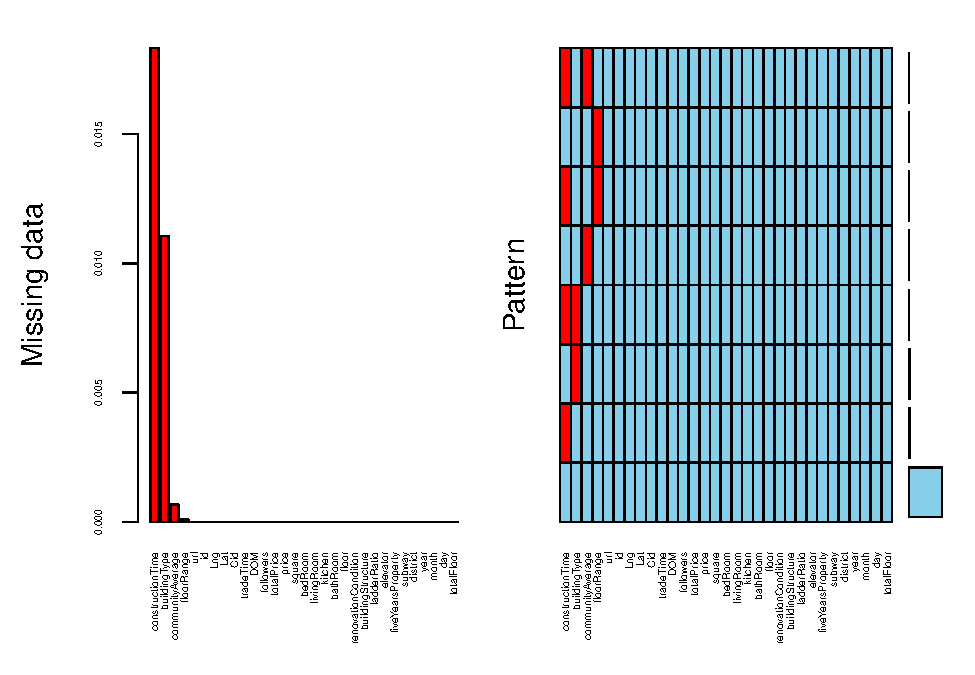
\includegraphics{Project_files/figure-latex/unnamed-chunk-6-1.pdf}

\begin{verbatim}
## 
##  Variables sorted by number of missings: 
##             Variable        Count
##     constructionTime 1.832612e-02
##         buildingType 1.106046e-02
##     communityAverage 6.710322e-04
##           floorRange 9.255617e-05
##                  url 0.000000e+00
##                   id 0.000000e+00
##                  Lng 0.000000e+00
##                  Lat 0.000000e+00
##                  Cid 0.000000e+00
##            tradeTime 0.000000e+00
##                  DOM 0.000000e+00
##            followers 0.000000e+00
##           totalPrice 0.000000e+00
##                price 0.000000e+00
##               square 0.000000e+00
##              bedRoom 0.000000e+00
##           livingRoom 0.000000e+00
##              kitchen 0.000000e+00
##             bathRoom 0.000000e+00
##                floor 0.000000e+00
##  renovationCondition 0.000000e+00
##    buildingStructure 0.000000e+00
##          ladderRatio 0.000000e+00
##             elevator 0.000000e+00
##    fiveYearsProperty 0.000000e+00
##               subway 0.000000e+00
##             district 0.000000e+00
##                 year 0.000000e+00
##                month 0.000000e+00
##                  day 0.000000e+00
##           totalFloor 0.000000e+00
\end{verbatim}

Our data had 1303 missing values. All missing values are in variables
construction time, building type, community average, and floor range.
The above graph shows the proportion of missing values in each variable
with the highest being 0.018 for construction time. \newline We decided
to remove all missing values for two reasons. First, 1303 missing values
is a relatively small amount of data compared to 43217 observations we
have. Second, we did not plan to use the variable buildingType and
community average, which had a large portion of missing values.

\begin{Shaded}
\begin{Highlighting}[]
\NormalTok{data2017 }\OtherTok{\textless{}{-}} \FunctionTok{na.omit}\NormalTok{(data2017)}
\end{Highlighting}
\end{Shaded}

Now we have 42710 observations.

\hypertarget{remove-unnecessary-variables}{%
\subsection{2.5 Remove unnecessary
variables}\label{remove-unnecessary-variables}}

The final step of data cleaning is removing variables that we do not
plan to use.

\begin{Shaded}
\begin{Highlighting}[]
\NormalTok{data2017 }\OtherTok{\textless{}{-}}\NormalTok{ data2017 }\SpecialCharTok{\%\textgreater{}\%}
  \FunctionTok{select}\NormalTok{(}\SpecialCharTok{{-}}\FunctionTok{c}\NormalTok{(url, Lng, Lat, Cid, tradeTime, floor, buildingType, communityAverage, year))}
\end{Highlighting}
\end{Shaded}

\hypertarget{section-3-exploratory-analysis}{%
\section{Section 3: Exploratory
Analysis}\label{section-3-exploratory-analysis}}

\hypertarget{distribution-of-variables-and-outliers}{%
\subsection{3.1 Distribution of variables and
outliers}\label{distribution-of-variables-and-outliers}}

\hypertarget{month}{%
\subsubsection{3.1.1 Month}\label{month}}

\begin{Shaded}
\begin{Highlighting}[]
\FunctionTok{ggplot}\NormalTok{(data2017, }\FunctionTok{aes}\NormalTok{(}\AttributeTok{x =}\NormalTok{ month)) }\SpecialCharTok{+} 
  \FunctionTok{geom\_bar}\NormalTok{(}\AttributeTok{fill =} \StringTok{"light blue"}\NormalTok{) }\SpecialCharTok{+} 
  \FunctionTok{scale\_x\_discrete}\NormalTok{(}\AttributeTok{limits =}\NormalTok{ month.name)}
\end{Highlighting}
\end{Shaded}

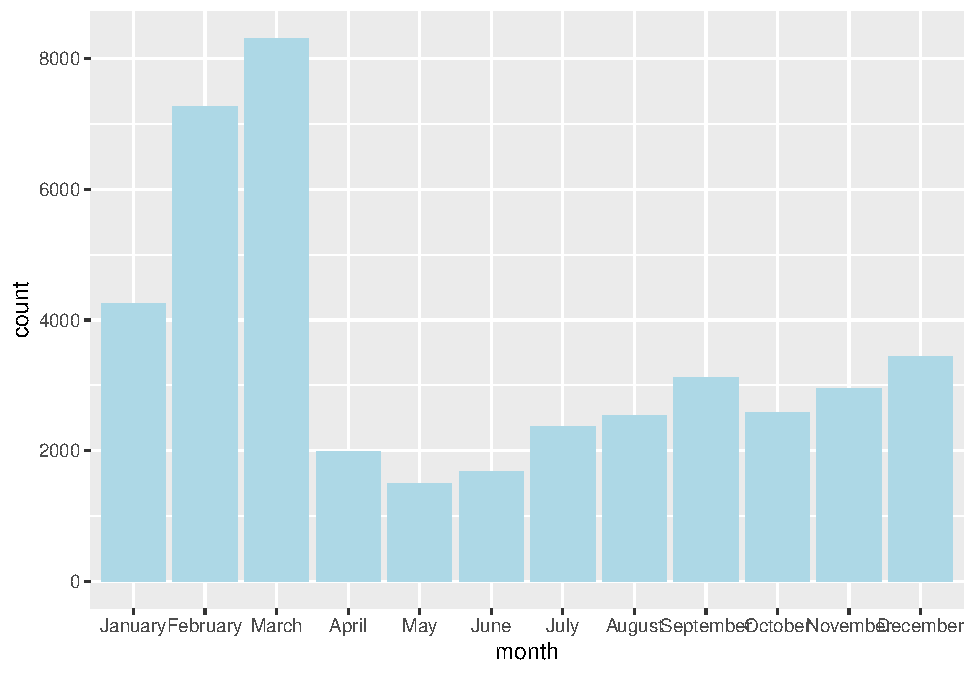
\includegraphics{Project_files/figure-latex/unnamed-chunk-9-1.pdf}

The first three months of year 2017 had the most trading of houses, with
March being the highest number of trading, more than 8000 tradings.
Apirl, May, and June each only had less than 1/4 of the number of
trading compared to March. The amount of transactions for the rest of
the year remained below 4000.

\hypertarget{day}{%
\subsubsection{3.1.2 Day}\label{day}}

\begin{Shaded}
\begin{Highlighting}[]
\FunctionTok{ggplot}\NormalTok{(data2017, }\FunctionTok{aes}\NormalTok{(}\AttributeTok{x =}\NormalTok{ day)) }\SpecialCharTok{+} 
  \FunctionTok{geom\_bar}\NormalTok{(}\AttributeTok{fill =} \StringTok{"light blue"}\NormalTok{, }\AttributeTok{color =} \StringTok{"black"}\NormalTok{)}
\end{Highlighting}
\end{Shaded}

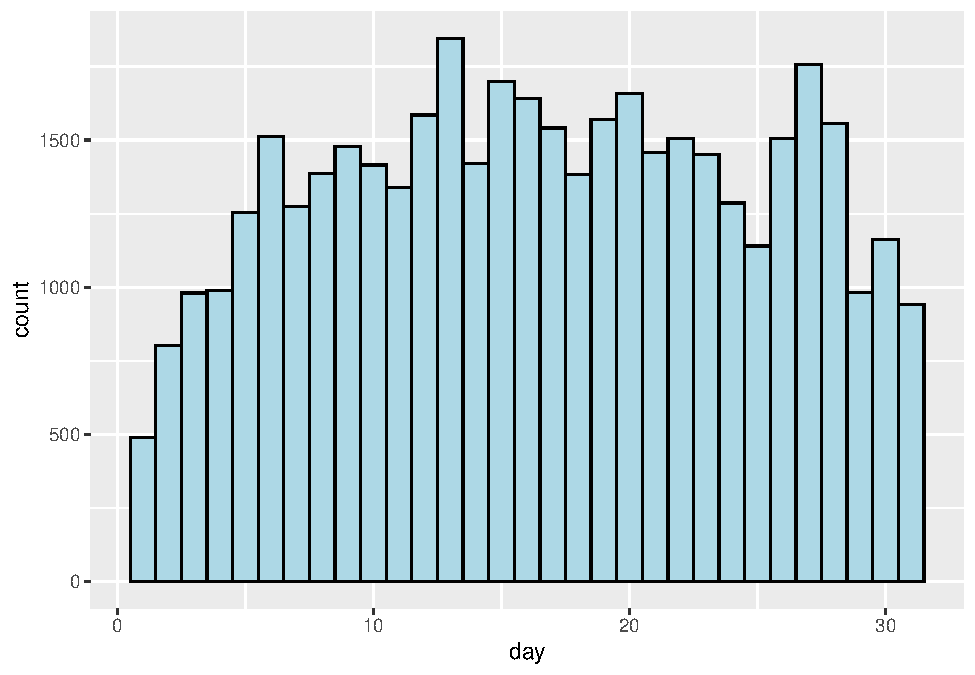
\includegraphics{Project_files/figure-latex/unnamed-chunk-10-1.pdf}
There isn't a unique day of the month that people liked to buy houses,
but people relatively like to buy houses in the middle of the month. Few
trades happened in the beginning of the month.

\hypertarget{total-floor}{%
\subsubsection{3.1.3 Total Floor}\label{total-floor}}

\begin{Shaded}
\begin{Highlighting}[]
\FunctionTok{ggplot}\NormalTok{(data2017, }\FunctionTok{aes}\NormalTok{(}\AttributeTok{x =}\NormalTok{ totalFloor)) }\SpecialCharTok{+} \FunctionTok{geom\_histogram}\NormalTok{(}\AttributeTok{color =} \StringTok{"black"}\NormalTok{, }\AttributeTok{fill =} \StringTok{"blue"}\NormalTok{) }
\end{Highlighting}
\end{Shaded}

\begin{verbatim}
## `stat_bin()` using `bins = 30`. Pick better value with `binwidth`.
\end{verbatim}

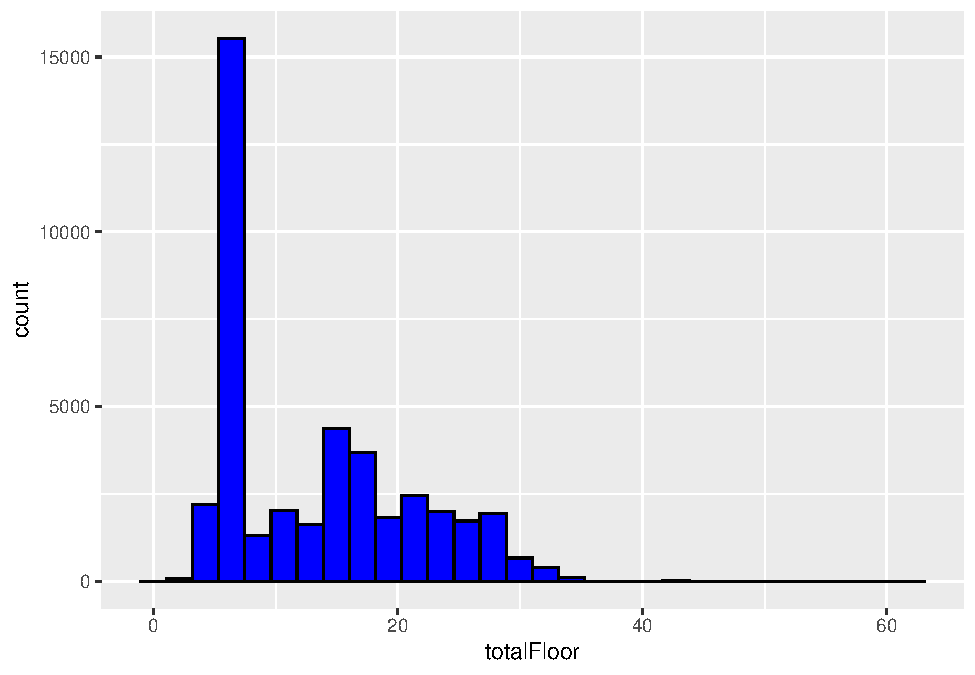
\includegraphics{Project_files/figure-latex/unnamed-chunk-11-1.pdf}

\begin{Shaded}
\begin{Highlighting}[]
\FunctionTok{summary}\NormalTok{(data2017}\SpecialCharTok{$}\NormalTok{totalFloor)}
\end{Highlighting}
\end{Shaded}

\begin{verbatim}
##    Min. 1st Qu.  Median    Mean 3rd Qu.    Max. 
##    1.00    6.00   11.00   13.38   20.00   63.00
\end{verbatim}

\begin{Shaded}
\begin{Highlighting}[]
\NormalTok{data2017 }\SpecialCharTok{\%\textgreater{}\%} \FunctionTok{arrange}\NormalTok{(}\FunctionTok{desc}\NormalTok{(totalFloor)) }\SpecialCharTok{\%\textgreater{}\%} \FunctionTok{select}\NormalTok{(id, totalFloor, floorRange) }\SpecialCharTok{\%\textgreater{}\%} \FunctionTok{head}\NormalTok{()}
\end{Highlighting}
\end{Shaded}

\begin{verbatim}
##             id totalFloor floorRange
## 1 101101127418         63        low
## 2 101101690389         57     midium
## 3 101091696453         42        low
## 4 101100641538         42        low
## 5 101100768834         42       high
## 6 101100791635         42     midium
\end{verbatim}

\begin{Shaded}
\begin{Highlighting}[]
\NormalTok{data2017 }\OtherTok{\textless{}{-}}\NormalTok{ data2017 }\SpecialCharTok{\%\textgreater{}\%}
  \FunctionTok{filter}\NormalTok{(totalFloor }\SpecialCharTok{\textless{}} \DecValTok{60}\NormalTok{)}
\end{Highlighting}
\end{Shaded}

The distribution of total floor is unimodel and skewed to the right.
There are quite a few very tall buildings, but such high numbers could
be an error in data recording. The url for the apartment located in a
building with 63 floors is invalid; however, we checked the apartment
located in the building with 57 floors using url and, surprisingly, the
building does exist and is called Yu Jin Tai. Therefore, we only removed
the trade with total floor of 63.

\hypertarget{floor-range}{%
\subsubsection{3.1.4 Floor Range}\label{floor-range}}

\begin{Shaded}
\begin{Highlighting}[]
\FunctionTok{ggplot}\NormalTok{(data2017, }\FunctionTok{aes}\NormalTok{(}\AttributeTok{x =}\NormalTok{ floorRange)) }\SpecialCharTok{+} 
  \FunctionTok{geom\_bar}\NormalTok{(}\AttributeTok{fill =} \StringTok{"light blue"}\NormalTok{) }\SpecialCharTok{+}
  \FunctionTok{scale\_x\_discrete}\NormalTok{(}\AttributeTok{limits =} \FunctionTok{c}\NormalTok{(}\StringTok{"bottom"}\NormalTok{, }\StringTok{"low"}\NormalTok{, }\StringTok{"midium"}\NormalTok{, }\StringTok{"high"}\NormalTok{, }\StringTok{"top"}\NormalTok{)) }
\end{Highlighting}
\end{Shaded}

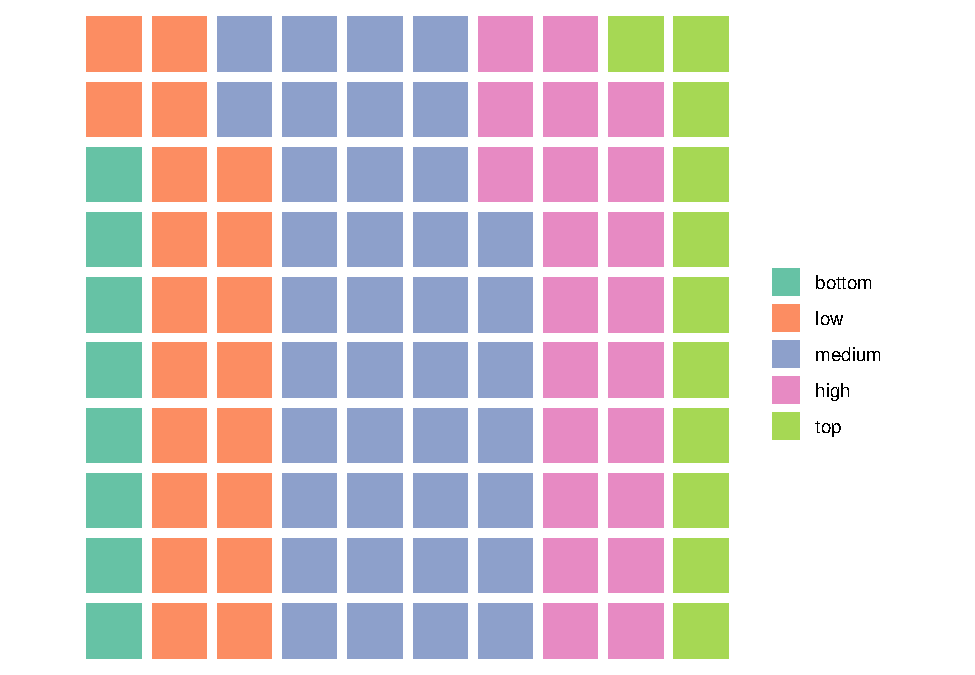
\includegraphics{Project_files/figure-latex/unnamed-chunk-12-1.pdf}
Apartments located in the middle of a building were traded the most in
2017.

\hypertarget{dom}{%
\subsubsection{3.1.5 DOM}\label{dom}}

The graph of number of days on market is unimodal and heavily skewed to
the right. The mean number of days on market is around 51 and the median
is 31 days. Approximately 2.5\% of values are below 2. Approximately
2.5\% of values are above 196. The longest day on market is 721. Whereas
there are total of 474 houses have less or equal to 1 day on market
until sold.

\begin{Shaded}
\begin{Highlighting}[]
\FunctionTok{ggplot}\NormalTok{(data2017, }\FunctionTok{aes}\NormalTok{(}\AttributeTok{x=}\NormalTok{DOM))}\SpecialCharTok{+}
  \FunctionTok{geom\_histogram}\NormalTok{(}\AttributeTok{fill=}\StringTok{\textquotesingle{}lightblue\textquotesingle{}}\NormalTok{, }\AttributeTok{color=}\StringTok{\textquotesingle{}black\textquotesingle{}}\NormalTok{) }\SpecialCharTok{+}
  \FunctionTok{xlab}\NormalTok{(}\StringTok{"DOM"}\NormalTok{)}\SpecialCharTok{+}\FunctionTok{ylab}\NormalTok{(}\StringTok{"Count"}\NormalTok{)}\SpecialCharTok{+}\FunctionTok{ggtitle}\NormalTok{(}\StringTok{"Active Days on Market Histogram"}\NormalTok{)}
\end{Highlighting}
\end{Shaded}

\begin{verbatim}
## `stat_bin()` using `bins = 30`. Pick better value with `binwidth`.
\end{verbatim}

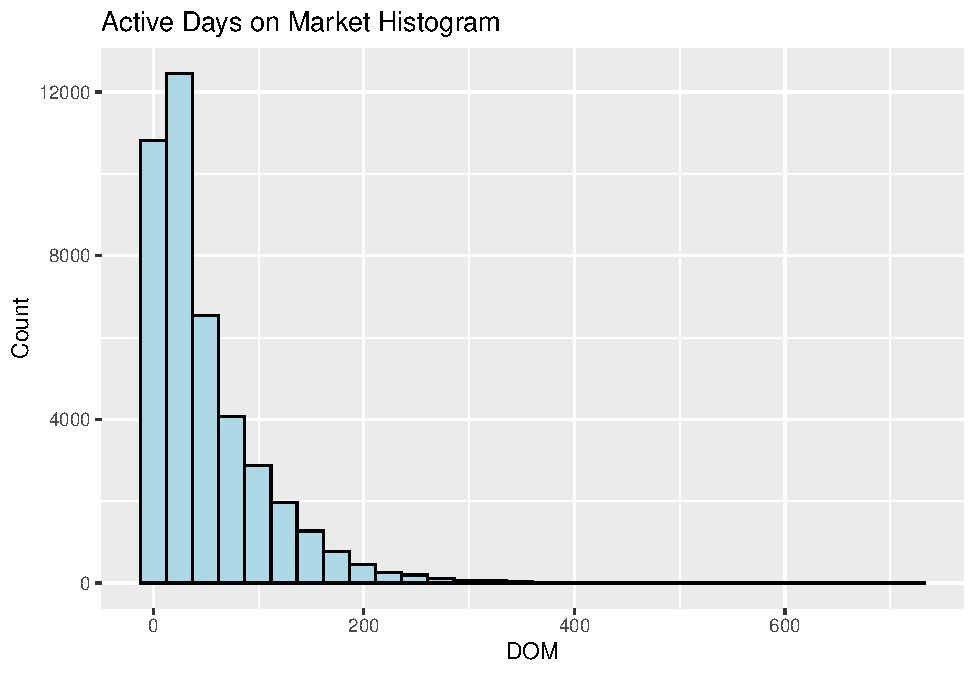
\includegraphics{Project_files/figure-latex/unnamed-chunk-13-1.pdf}

\begin{Shaded}
\begin{Highlighting}[]
\FunctionTok{mean}\NormalTok{(data2017}\SpecialCharTok{$}\NormalTok{DOM)}
\end{Highlighting}
\end{Shaded}

\begin{verbatim}
## [1] 50.858
\end{verbatim}

\begin{Shaded}
\begin{Highlighting}[]
\FunctionTok{quantile}\NormalTok{(data2017}\SpecialCharTok{$}\NormalTok{DOM, }\FunctionTok{c}\NormalTok{(}\DecValTok{0}\NormalTok{, }\FloatTok{0.025}\NormalTok{, }\FloatTok{0.25}\NormalTok{, }\FloatTok{0.5}\NormalTok{, }\FloatTok{0.75}\NormalTok{, }\FloatTok{0.975}\NormalTok{, }\DecValTok{1}\NormalTok{))}
\end{Highlighting}
\end{Shaded}

\begin{verbatim}
##    0%  2.5%   25%   50%   75% 97.5%  100% 
##     1     2    12    31    71   196   721
\end{verbatim}

\begin{Shaded}
\begin{Highlighting}[]
\NormalTok{data2017 }\SpecialCharTok{\%\textgreater{}\%}
  \FunctionTok{filter}\NormalTok{(DOM}\SpecialCharTok{\textless{}=}\DecValTok{1}\NormalTok{) }\SpecialCharTok{\%\textgreater{}\%}
  \FunctionTok{nrow}\NormalTok{()  }\CommentTok{\# number of houses have less than 1 day on market}
\end{Highlighting}
\end{Shaded}

\begin{verbatim}
## [1] 474
\end{verbatim}

\hypertarget{followers}{%
\subsubsection{3.1.6 followers}\label{followers}}

The graph of number of followers is unimodal and heavily skewed to the
right. The mean is around 49 people and the median is around 31 people.
Approximately 2.5\% of values are below or equal to 0. Approximately
2.5\% of values are above 216. However, the highest 2.5\% are jumps from
216 to 1143, which suggests that there are a few significantly popular
houses. There are 5617 houses with 0 follower and also a total of 5
houses with more than 1000 followers. Among these houses with more than
1000 followers, 1 house has significant low total price compare with
other houses. However, it also has relative small area and is located in
the suburb, which makes this reasonable.

\begin{Shaded}
\begin{Highlighting}[]
\FunctionTok{ggplot}\NormalTok{(data2017, }\FunctionTok{aes}\NormalTok{(}\AttributeTok{x=}\NormalTok{followers))}\SpecialCharTok{+}
  \FunctionTok{geom\_histogram}\NormalTok{(}\AttributeTok{fill=}\StringTok{\textquotesingle{}lightblue\textquotesingle{}}\NormalTok{, }\AttributeTok{color=}\StringTok{\textquotesingle{}black\textquotesingle{}}\NormalTok{) }\SpecialCharTok{+}
  \FunctionTok{xlab}\NormalTok{(}\StringTok{"followers"}\NormalTok{)}\SpecialCharTok{+}\FunctionTok{ylab}\NormalTok{(}\StringTok{"Count"}\NormalTok{)}\SpecialCharTok{+}
  \FunctionTok{ggtitle}\NormalTok{(}\StringTok{"followers Histogram"}\NormalTok{)}
\end{Highlighting}
\end{Shaded}

\begin{verbatim}
## `stat_bin()` using `bins = 30`. Pick better value with `binwidth`.
\end{verbatim}

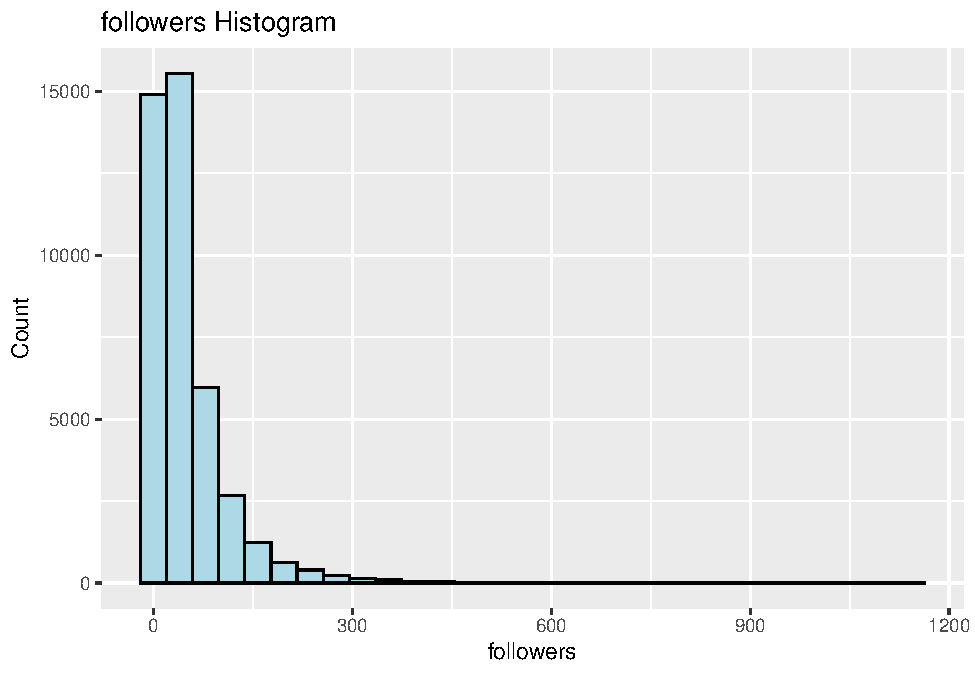
\includegraphics{Project_files/figure-latex/unnamed-chunk-14-1.pdf}

\begin{Shaded}
\begin{Highlighting}[]
\FunctionTok{mean}\NormalTok{(data2017}\SpecialCharTok{$}\NormalTok{followers)}
\end{Highlighting}
\end{Shaded}

\begin{verbatim}
## [1] 49.41241
\end{verbatim}

\begin{Shaded}
\begin{Highlighting}[]
\FunctionTok{quantile}\NormalTok{(data2017}\SpecialCharTok{$}\NormalTok{followers, }\FunctionTok{c}\NormalTok{(}\DecValTok{0}\NormalTok{, }\FloatTok{0.025}\NormalTok{, }\FloatTok{0.25}\NormalTok{, }\FloatTok{0.5}\NormalTok{, }\FloatTok{0.75}\NormalTok{, }\FloatTok{0.975}\NormalTok{, }\DecValTok{1}\NormalTok{))}
\end{Highlighting}
\end{Shaded}

\begin{verbatim}
##    0%  2.5%   25%   50%   75% 97.5%  100% 
##     0     0    11    31    64   216  1143
\end{verbatim}

\begin{Shaded}
\begin{Highlighting}[]
\NormalTok{data2017 }\SpecialCharTok{\%\textgreater{}\%} \FunctionTok{filter}\NormalTok{(followers}\SpecialCharTok{\textgreater{}}\DecValTok{1000}\NormalTok{)}
\end{Highlighting}
\end{Shaded}

\begin{verbatim}
##             id DOM followers totalPrice  price square bedRoom livingRoom
## 1 101100732988 132      1085       48.0  26667  18.00       1          1
## 2 101100746033 141      1015      297.5  78393  37.95       1          0
## 3 101101590746 229      1143      380.0 116780  32.54       1          1
## 4 101102303199  25      1045      514.0  87415  58.80       2          1
##   kitchen bathRoom constructionTime renovationCondition buildingStructure
## 1       1        1             2011                   4                 6
## 2       1        1             2007                   4                 6
## 3       1        2             2005                   3                 6
## 4       1        1             1992                   4                 2
##   ladderRatio elevator fiveYearsProperty subway  district    month day
## 1       0.385        1                 0      0 ChangPing February  24
## 2       0.250        1                 1      1  ChaoYang    March   9
## 3       0.077        1                 1      1   XiCheng December  31
## 4       0.500        0                 1      1   HaiDian December   8
##   totalFloor floorRange
## 1         28     midium
## 2         12       high
## 3         10     midium
## 4          6       high
\end{verbatim}

\hypertarget{totalprice}{%
\subsubsection{3.1.7 totalPrice}\label{totalprice}}

The graph of total price is diamond-shaped, unimodal, and skews right.
The average total price of a house in Beijing in 2017 is 526x10,000 yuan
(around 750\textasciitilde810 thousands dollars depend on inflation) and
the median is 460x10,000 yuan (around 660\textasciitilde710 thousands
dollars). Approximately 2.5\% of values are below 215x10,000 yuan.
Approximately 2.5\% of values are above 1250x10,000 yuan.

\begin{Shaded}
\begin{Highlighting}[]
\FunctionTok{ggplot}\NormalTok{(data2017, }\FunctionTok{aes}\NormalTok{(}\AttributeTok{x=}\NormalTok{totalPrice))}\SpecialCharTok{+}
  \FunctionTok{geom\_histogram}\NormalTok{(}\AttributeTok{fill=}\StringTok{\textquotesingle{}lightblue\textquotesingle{}}\NormalTok{, }\AttributeTok{color=}\StringTok{\textquotesingle{}black\textquotesingle{}}\NormalTok{) }\SpecialCharTok{+}
  \FunctionTok{xlab}\NormalTok{(}\StringTok{"totalPrice"}\NormalTok{)}\SpecialCharTok{+}\FunctionTok{ylab}\NormalTok{(}\StringTok{"Count"}\NormalTok{)}\SpecialCharTok{+}\FunctionTok{ggtitle}\NormalTok{(}\StringTok{"Total price (in 10,000yuan) Histogram"}\NormalTok{)}
\end{Highlighting}
\end{Shaded}

\begin{verbatim}
## `stat_bin()` using `bins = 30`. Pick better value with `binwidth`.
\end{verbatim}

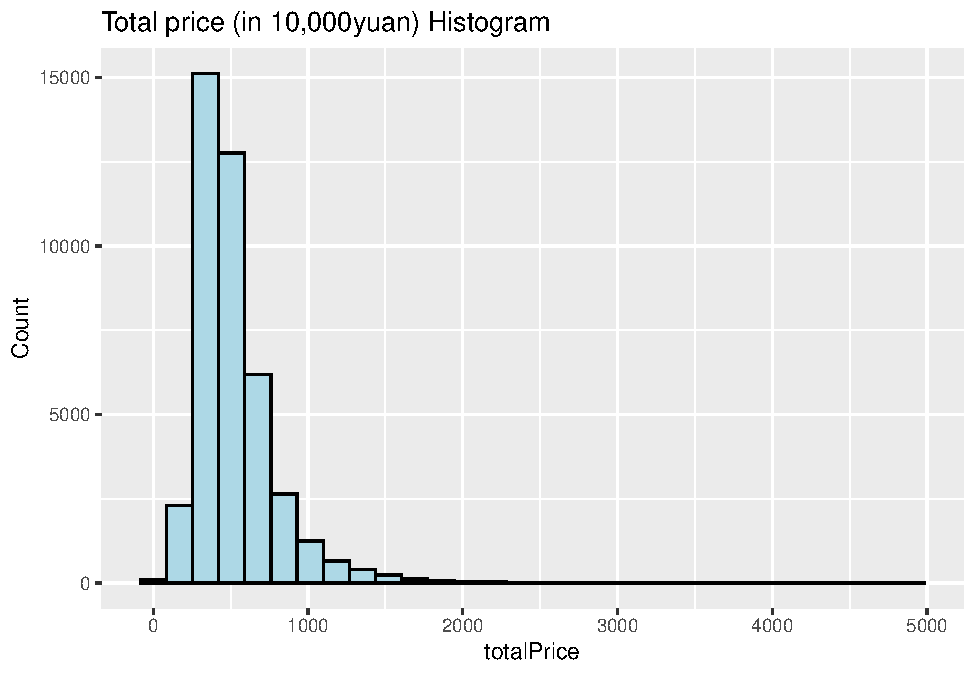
\includegraphics{Project_files/figure-latex/unnamed-chunk-15-1.pdf}

\begin{Shaded}
\begin{Highlighting}[]
\FunctionTok{mean}\NormalTok{(data2017}\SpecialCharTok{$}\NormalTok{totalPrice)}
\end{Highlighting}
\end{Shaded}

\begin{verbatim}
## [1] 526.3465
\end{verbatim}

\begin{Shaded}
\begin{Highlighting}[]
\FunctionTok{quantile}\NormalTok{(data2017}\SpecialCharTok{$}\NormalTok{totalPrice, }\FunctionTok{c}\NormalTok{(}\DecValTok{0}\NormalTok{, }\FloatTok{0.025}\NormalTok{, }\FloatTok{0.25}\NormalTok{, }\FloatTok{0.5}\NormalTok{, }\FloatTok{0.75}\NormalTok{, }\FloatTok{0.975}\NormalTok{, }\DecValTok{1}\NormalTok{))}
\end{Highlighting}
\end{Shaded}

\begin{verbatim}
##     0%   2.5%    25%    50%    75%  97.5%   100% 
##    1.0  215.5  355.0  460.0  616.0 1250.0 4900.0
\end{verbatim}

\begin{Shaded}
\begin{Highlighting}[]
\FunctionTok{ggplot}\NormalTok{(data2017, }\FunctionTok{aes}\NormalTok{(}\AttributeTok{x=}\NormalTok{district,}\AttributeTok{y=}\NormalTok{totalPrice))}\SpecialCharTok{+}
  \FunctionTok{geom\_boxplot}\NormalTok{()}\SpecialCharTok{+}
  \FunctionTok{theme}\NormalTok{(}\AttributeTok{axis.text.x =} \FunctionTok{element\_text}\NormalTok{(}\AttributeTok{angle =} \DecValTok{45}\NormalTok{, }\AttributeTok{vjust =} \FloatTok{0.5}\NormalTok{, }\AttributeTok{hjust=}\DecValTok{1}\NormalTok{))}
\end{Highlighting}
\end{Shaded}

\includegraphics{Project_files/figure-latex/unnamed-chunk-15-2.pdf}

\hypertarget{price}{%
\subsubsection{3.1.8 price}\label{price}}

The graph for price is Diamond-shaped, unimodal, and skewed right. The
average price per square meter is around 67,430 yuan and median is
62,670 yuan, which are close. Approximately 2.5\% of values are above
127,359 yuan. Approximately 2.5\% of values are below 33,035 yuan. The
house that has the lowest value has 136 yuan per square meter, which is
about 20 dollars per square meter. Such low price doesn't make sense in
any part of Beijing. Therefore, we decided to remove this outlier.

\begin{Shaded}
\begin{Highlighting}[]
\FunctionTok{ggplot}\NormalTok{(data2017, }\FunctionTok{aes}\NormalTok{(}\AttributeTok{x=}\NormalTok{price))}\SpecialCharTok{+}
  \FunctionTok{geom\_histogram}\NormalTok{(}\AttributeTok{fill=}\StringTok{\textquotesingle{}lightblue\textquotesingle{}}\NormalTok{, }\AttributeTok{color=}\StringTok{\textquotesingle{}black\textquotesingle{}}\NormalTok{) }\SpecialCharTok{+}
  \FunctionTok{xlab}\NormalTok{(}\StringTok{"price"}\NormalTok{)}\SpecialCharTok{+}\FunctionTok{ylab}\NormalTok{(}\StringTok{"Count"}\NormalTok{)}\SpecialCharTok{+}\FunctionTok{ggtitle}\NormalTok{(}\StringTok{"Average price per square meter (in yuan) Histogram"}\NormalTok{)}
\end{Highlighting}
\end{Shaded}

\begin{verbatim}
## `stat_bin()` using `bins = 30`. Pick better value with `binwidth`.
\end{verbatim}

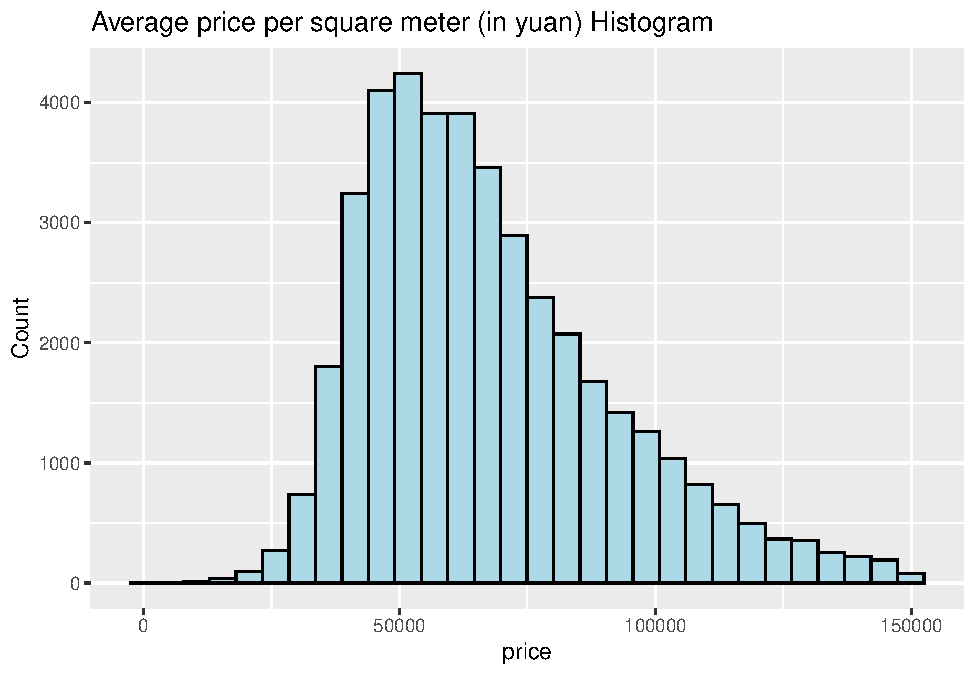
\includegraphics{Project_files/figure-latex/unnamed-chunk-16-1.pdf}

\begin{Shaded}
\begin{Highlighting}[]
\FunctionTok{mean}\NormalTok{(data2017}\SpecialCharTok{$}\NormalTok{price)}
\end{Highlighting}
\end{Shaded}

\begin{verbatim}
## [1] 67428.99
\end{verbatim}

\begin{Shaded}
\begin{Highlighting}[]
\FunctionTok{quantile}\NormalTok{(data2017}\SpecialCharTok{$}\NormalTok{price, }\FunctionTok{c}\NormalTok{(}\DecValTok{0}\NormalTok{, }\FloatTok{0.025}\NormalTok{, }\FloatTok{0.25}\NormalTok{, }\FloatTok{0.5}\NormalTok{, }\FloatTok{0.75}\NormalTok{, }\FloatTok{0.975}\NormalTok{, }\DecValTok{1}\NormalTok{))}
\end{Highlighting}
\end{Shaded}

\begin{verbatim}
##        0%      2.5%       25%       50%       75%     97.5%      100% 
##    136.00  33034.15  49330.00  62669.00  81075.50 127358.70 150000.00
\end{verbatim}

\begin{Shaded}
\begin{Highlighting}[]
\NormalTok{data2017 }\SpecialCharTok{\%\textgreater{}\%}
  \FunctionTok{filter}\NormalTok{(price}\SpecialCharTok{\textless{}=}\DecValTok{1000}\NormalTok{) }
\end{Highlighting}
\end{Shaded}

\begin{verbatim}
##             id DOM followers totalPrice price square bedRoom livingRoom kitchen
## 1 101101646066   2         0          1   136   73.8       2          1       1
##   bathRoom constructionTime renovationCondition buildingStructure ladderRatio
## 1        1             1993                   1                 6         0.2
##   elevator fiveYearsProperty subway district month day totalFloor floorRange
## 1        1                 0      0  HaiDian  June   2         18     bottom
\end{verbatim}

\begin{Shaded}
\begin{Highlighting}[]
\NormalTok{data2017 }\OtherTok{\textless{}{-}}\NormalTok{ data2017 }\SpecialCharTok{\%\textgreater{}\%} 
  \FunctionTok{filter}\NormalTok{(price}\SpecialCharTok{\textgreater{}}\DecValTok{1000}\NormalTok{)}

\FunctionTok{summary}\NormalTok{(data2017}\SpecialCharTok{$}\NormalTok{price)}
\end{Highlighting}
\end{Shaded}

\begin{verbatim}
##    Min. 1st Qu.  Median    Mean 3rd Qu.    Max. 
##    1194   49333   62670   67431   81076  150000
\end{verbatim}

\begin{Shaded}
\begin{Highlighting}[]
\FunctionTok{ggplot}\NormalTok{(data2017, }\FunctionTok{aes}\NormalTok{(}\AttributeTok{x=}\NormalTok{district,}\AttributeTok{y=}\NormalTok{price))}\SpecialCharTok{+}
  \FunctionTok{geom\_boxplot}\NormalTok{()}\SpecialCharTok{+}
  \FunctionTok{theme}\NormalTok{(}\AttributeTok{axis.text.x =} \FunctionTok{element\_text}\NormalTok{(}\AttributeTok{angle =} \DecValTok{45}\NormalTok{, }\AttributeTok{vjust =} \FloatTok{0.5}\NormalTok{, }\AttributeTok{hjust=}\DecValTok{1}\NormalTok{))}
\end{Highlighting}
\end{Shaded}

\includegraphics{Project_files/figure-latex/unnamed-chunk-16-2.pdf}

\hypertarget{square}{%
\subsubsection{3.1.9 square}\label{square}}

The graph of number of squares is diamond-shaped, unimodal, and skews
right. The mean of houses sold in Beijing in 2017 have around 81 square
meters. The median is around 72 square meters. Approximately 2.5\% of
values are below 37 square meters. Approximately 2.5\% of values are
above 167 square meters.

\begin{Shaded}
\begin{Highlighting}[]
\FunctionTok{ggplot}\NormalTok{(data2017, }\FunctionTok{aes}\NormalTok{(}\AttributeTok{x=}\NormalTok{square))}\SpecialCharTok{+}
  \FunctionTok{geom\_histogram}\NormalTok{(}\AttributeTok{fill=}\StringTok{\textquotesingle{}lightblue\textquotesingle{}}\NormalTok{, }\AttributeTok{color=}\StringTok{\textquotesingle{}black\textquotesingle{}}\NormalTok{) }\SpecialCharTok{+}
  \FunctionTok{xlab}\NormalTok{(}\StringTok{"square"}\NormalTok{)}\SpecialCharTok{+}\FunctionTok{ylab}\NormalTok{(}\StringTok{"Count"}\NormalTok{)}\SpecialCharTok{+}\FunctionTok{ggtitle}\NormalTok{(}\StringTok{"square of the House Histogram"}\NormalTok{) }
\end{Highlighting}
\end{Shaded}

\begin{verbatim}
## `stat_bin()` using `bins = 30`. Pick better value with `binwidth`.
\end{verbatim}

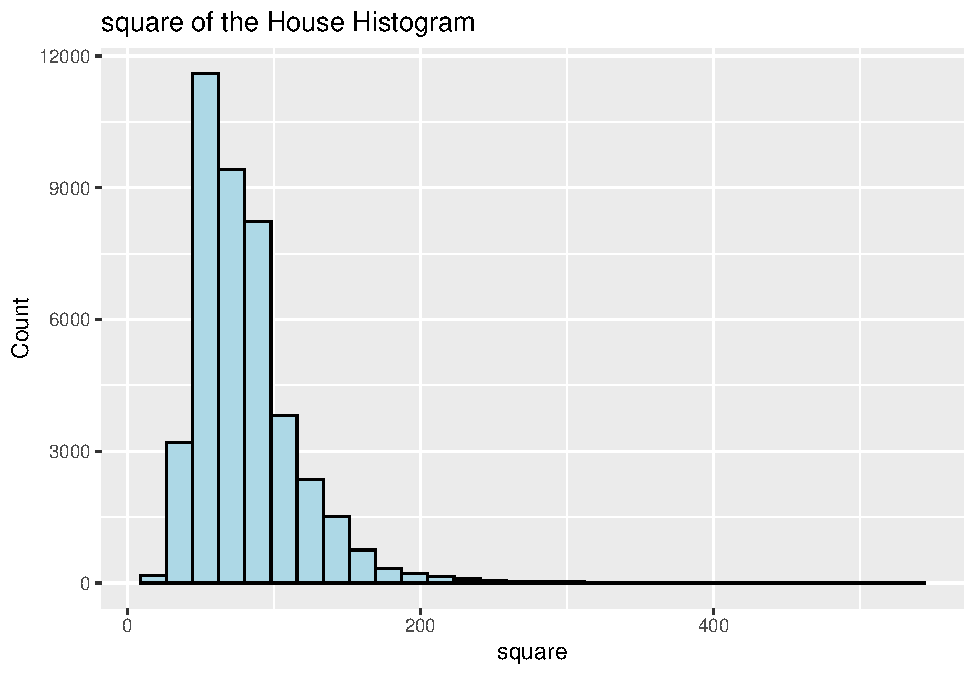
\includegraphics{Project_files/figure-latex/unnamed-chunk-17-1.pdf}

\begin{Shaded}
\begin{Highlighting}[]
\FunctionTok{mean}\NormalTok{(data2017}\SpecialCharTok{$}\NormalTok{square)}
\end{Highlighting}
\end{Shaded}

\begin{verbatim}
## [1] 80.9039
\end{verbatim}

\begin{Shaded}
\begin{Highlighting}[]
\FunctionTok{quantile}\NormalTok{(data2017}\SpecialCharTok{$}\NormalTok{square, }\FunctionTok{c}\NormalTok{(}\DecValTok{0}\NormalTok{, }\FloatTok{0.025}\NormalTok{, }\FloatTok{0.25}\NormalTok{, }\FloatTok{0.5}\NormalTok{, }\FloatTok{0.75}\NormalTok{, }\FloatTok{0.975}\NormalTok{, }\DecValTok{1}\NormalTok{))}
\end{Highlighting}
\end{Shaded}

\begin{verbatim}
##       0%     2.5%      25%      50%      75%    97.5%     100% 
##  15.0000  37.2725  57.3800  72.3600  95.0600 166.5900 532.2500
\end{verbatim}

A house with more 1745.5 square meter seems very unreasonable, so we
decided houses that are less than 1000 square meters are plausible.

\begin{Shaded}
\begin{Highlighting}[]
\NormalTok{data2017 }\OtherTok{\textless{}{-}}\NormalTok{ data2017 }\SpecialCharTok{\%\textgreater{}\%} 
  \FunctionTok{filter}\NormalTok{(square }\SpecialCharTok{\textless{}} \DecValTok{1000}\NormalTok{)}
\end{Highlighting}
\end{Shaded}

\hypertarget{bedroom}{%
\subsubsection{3.1.10 bedRoom}\label{bedroom}}

\hypertarget{might-be-a-report-error-move-the-house-with-0-bedroom-to-0-livingroom}{%
\subsection{might be a report error, move the house with 0 bedroom to 0
livingroom?}\label{might-be-a-report-error-move-the-house-with-0-bedroom-to-0-livingroom}}

One thing need to be noticed is that in this dataset, the variable
`livingRoom' could be understand as `bedroom' in the United States.
Thus, we decided to change the variable name from `livingRoom' to
`bedRoom'. The graph of number of bedrooms is unimodal, diamond-shaped,
and skews right. Most of the houses have 2 bedrooms, and the mean and
median number of bedrooms are both 2. Approximately 25\% of values are
below or equal to 1. Approximately 2.5\% of values are above 3.
(continued)

\begin{Shaded}
\begin{Highlighting}[]
\FunctionTok{ggplot}\NormalTok{(data2017, }\FunctionTok{aes}\NormalTok{(}\AttributeTok{x=}\NormalTok{bedRoom))}\SpecialCharTok{+}
  \FunctionTok{geom\_bar}\NormalTok{(}\AttributeTok{fill=}\StringTok{\textquotesingle{}lightblue\textquotesingle{}}\NormalTok{, }\AttributeTok{color=}\StringTok{\textquotesingle{}black\textquotesingle{}}\NormalTok{) }\SpecialCharTok{+} \CommentTok{\# use geom\_bar() instead of geom\_histogram()}
  \FunctionTok{xlab}\NormalTok{(}\StringTok{"bedRoom"}\NormalTok{)}\SpecialCharTok{+}\FunctionTok{ylab}\NormalTok{(}\StringTok{"Count"}\NormalTok{)}\SpecialCharTok{+}\FunctionTok{ggtitle}\NormalTok{(}\StringTok{"Number of bedroom Histogram"}\NormalTok{)}
\end{Highlighting}
\end{Shaded}

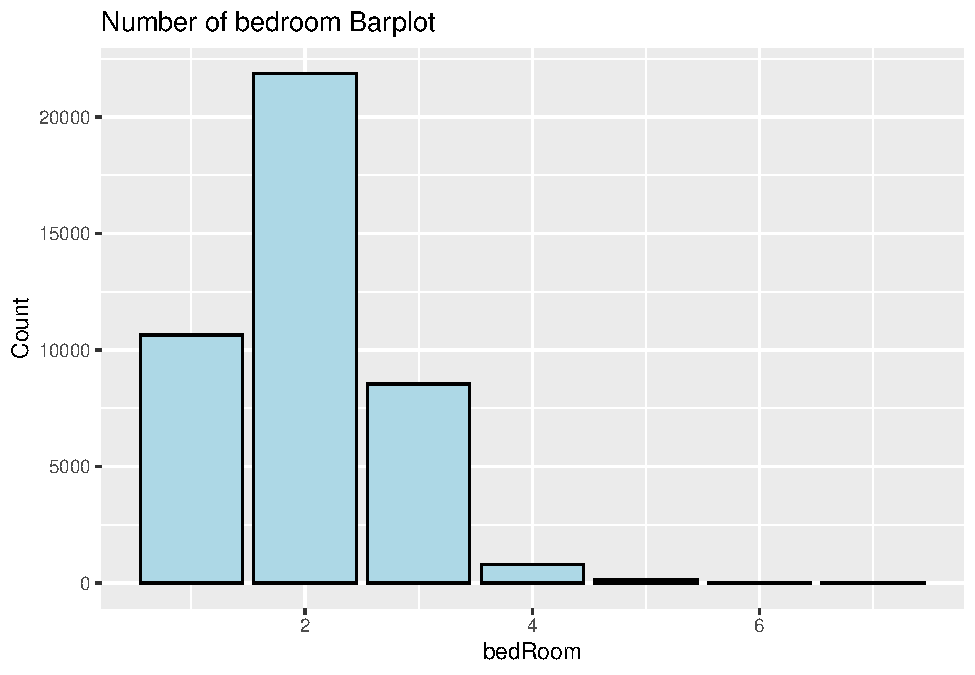
\includegraphics{Project_files/figure-latex/unnamed-chunk-19-1.pdf}

\begin{Shaded}
\begin{Highlighting}[]
\FunctionTok{mean}\NormalTok{(data2017}\SpecialCharTok{$}\NormalTok{bedRoom)}
\end{Highlighting}
\end{Shaded}

\begin{verbatim}
## [1] 2.000881
\end{verbatim}

\begin{Shaded}
\begin{Highlighting}[]
\FunctionTok{quantile}\NormalTok{(data2017}\SpecialCharTok{$}\NormalTok{bedRoom, }\FunctionTok{c}\NormalTok{(}\DecValTok{0}\NormalTok{, }\FloatTok{0.025}\NormalTok{, }\FloatTok{0.25}\NormalTok{, }\FloatTok{0.5}\NormalTok{, }\FloatTok{0.75}\NormalTok{, }\FloatTok{0.975}\NormalTok{, }\DecValTok{1}\NormalTok{))}
\end{Highlighting}
\end{Shaded}

\begin{verbatim}
##    0%  2.5%   25%   50%   75% 97.5%  100% 
##     0     1     1     2     2     3     7
\end{verbatim}

\begin{Shaded}
\begin{Highlighting}[]
\CommentTok{\# 1 house with 0 bed room}
\FunctionTok{table}\NormalTok{(data2017}\SpecialCharTok{$}\NormalTok{bedRoom)}
\end{Highlighting}
\end{Shaded}

\begin{verbatim}
## 
##     0     1     2     3     4     5     6     7 
##     1 10640 21859  8541   792   143    25     5
\end{verbatim}

\begin{Shaded}
\begin{Highlighting}[]
\NormalTok{data2017 }\SpecialCharTok{\%\textgreater{}\%}
  \FunctionTok{slice\_max}\NormalTok{(bedRoom,}\AttributeTok{n=}\DecValTok{1}\NormalTok{) }
\end{Highlighting}
\end{Shaded}

\begin{verbatim}
##             id DOM followers totalPrice price square bedRoom livingRoom kitchen
## 1 101100194821 257        77       2040 50000 408.00       7          3       1
## 2 101100882927 119        31       1690 52065 324.60       7          3       2
## 3 101100928521 251        94        700 20586 340.05       7          1       1
## 4 101101223183  17         5        840 58717 143.06       7          3       1
## 5 101101553400 100       168        678 24056 281.85       7          2       1
##   bathRoom constructionTime renovationCondition buildingStructure ladderRatio
## 1        3             2002                   4                 6       0.125
## 2        4             2001                   4                 6       0.250
## 3        2             2014                   2                 6       1.000
## 4        3             2011                   4                 6       0.500
## 5        3             2000                   4                 2       0.500
##   elevator fiveYearsProperty subway  district    month day totalFloor
## 1        0                 1      0   XiCheng February  28         24
## 2        1                 1      1  ChaoYang    March  24         22
## 3        1                 0      1    DaXing   August  13         24
## 4        1                 0      0 ChangPing    March  11          9
## 5        0                 1      0 ChangPing   August  14          6
##   floorRange
## 1        low
## 2     bottom
## 3     bottom
## 4     bottom
## 5     midium
\end{verbatim}

\begin{Shaded}
\begin{Highlighting}[]
\NormalTok{data2017 }\SpecialCharTok{\%\textgreater{}\%}
  \FunctionTok{slice\_min}\NormalTok{(bedRoom,}\AttributeTok{n=}\DecValTok{1}\NormalTok{)}
\end{Highlighting}
\end{Shaded}

\begin{verbatim}
##             id DOM followers totalPrice  price square bedRoom livingRoom
## 1 101101275312   3         0        450 145162     31       0          1
##   kitchen bathRoom constructionTime renovationCondition buildingStructure
## 1       1        1             2005                   1                 6
##   ladderRatio elevator fiveYearsProperty subway district month day totalFloor
## 1       0.081        1                 0      1  XiCheng March   6         10
##   floorRange
## 1     midium
\end{verbatim}

There is one house has 0 bedroom but sold in 145,612 yuan per square
meter which almost reached the highest square per meter sold among all
observations (150,000 yuan). Pulled out the link of this house, we found
that it is located in XiCheng. According to Lianjia website, this house
belongs to ``RongFeng 2008'' community. After a research on the
community, we found out that this is the average price per square meter
for this community. An investigation conducted by The Beijing News
indicates that ``RongFeng 2008'' has a relative 10,000 yuan higher price
per square meter compared with other communities in that area. But since
the houses in this community have very small areas, the total price is
still acceptable for most people who wanted to move to XiCheng. So this
house is not an outlier.

(\url{https://www.sohu.com/a/479132582_114988})

\begin{Shaded}
\begin{Highlighting}[]
\NormalTok{data }\SpecialCharTok{\%\textgreater{}\%}
  \FunctionTok{filter}\NormalTok{(id}\SpecialCharTok{==}\StringTok{"101101275312"}\NormalTok{)}
\end{Highlighting}
\end{Shaded}

\begin{verbatim}
##                                                  url           id      Lng
## 1 https://bj.lianjia.com/chengjiao/101101275312.html 101101275312 116.3432
##        Lat          Cid  tradeTime DOM followers totalPrice  price square
## 1 39.90053 1.111027e+12 2017-03-06   3         0        450 145162     31
##   livingRoom drawingRoom kitchen bathRoom floor buildingType constructionTime
## 1          0           1       1        1 中 10            1             2005
##   renovationCondition buildingStructure ladderRatio elevator fiveYearsProperty
## 1                   1                 6       0.081        1                 0
##   subway district communityAverage
## 1      1       10            92360
\end{verbatim}

\hypertarget{livingroom}{%
\subsubsection{3.1.11 livingRoom}\label{livingroom}}

The graph of number of living rooms is unimodal, diamond-shaped, and
skews right. The number of living rooms for all houses is between 0 to
4. Both the mean and median number of living rooms is 1. Approximately
2.5\% of values have no living room. Approximately 2.5\% of values have
more than 2 living rooms. Most houses sold in 2017 have 0 to 2 living
rooms and nearly 78\% of houses sold in 2017 have 1 living room. Houses
with 0 living room is the third greatest choice, and it is reasonable
for a house to have no living room, especially in the city.

\begin{Shaded}
\begin{Highlighting}[]
\FunctionTok{ggplot}\NormalTok{(data2017, }\FunctionTok{aes}\NormalTok{(}\AttributeTok{x=}\NormalTok{livingRoom))}\SpecialCharTok{+}
  \FunctionTok{geom\_bar}\NormalTok{(}\AttributeTok{fill=}\StringTok{\textquotesingle{}lightblue\textquotesingle{}}\NormalTok{, }\AttributeTok{color=}\StringTok{\textquotesingle{}black\textquotesingle{}}\NormalTok{) }\SpecialCharTok{+} \CommentTok{\# use geom\_bar() instead of geom\_histogram()}
  \FunctionTok{xlab}\NormalTok{(}\StringTok{"livingRoom"}\NormalTok{)}\SpecialCharTok{+}
  \FunctionTok{ylab}\NormalTok{(}\StringTok{"Count"}\NormalTok{)}\SpecialCharTok{+}
  \FunctionTok{ggtitle}\NormalTok{(}\StringTok{"Number of Living Rooms Histogram"}\NormalTok{)}
\end{Highlighting}
\end{Shaded}

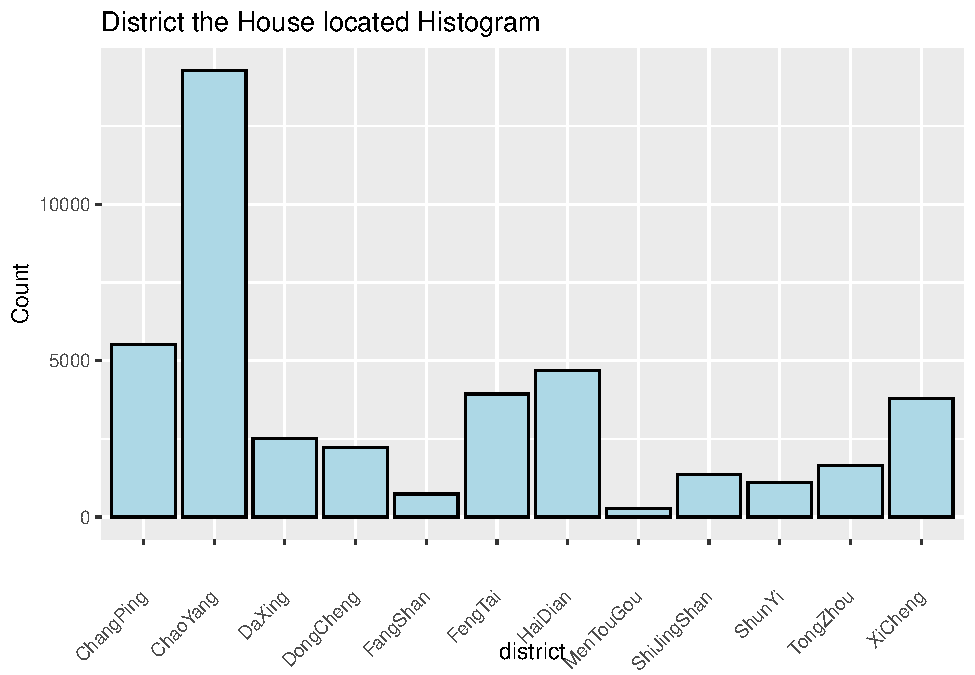
\includegraphics{Project_files/figure-latex/unnamed-chunk-21-1.pdf}

\begin{Shaded}
\begin{Highlighting}[]
\FunctionTok{mean}\NormalTok{(data2017}\SpecialCharTok{$}\NormalTok{livingRoom)}
\end{Highlighting}
\end{Shaded}

\begin{verbatim}
## [1] 1.09232
\end{verbatim}

\begin{Shaded}
\begin{Highlighting}[]
\FunctionTok{quantile}\NormalTok{(data2017}\SpecialCharTok{$}\NormalTok{livingRoom, }\FunctionTok{c}\NormalTok{(}\DecValTok{0}\NormalTok{, }\FloatTok{0.025}\NormalTok{, }\FloatTok{0.25}\NormalTok{, }\FloatTok{0.5}\NormalTok{, }\FloatTok{0.75}\NormalTok{, }\FloatTok{0.975}\NormalTok{, }\DecValTok{1}\NormalTok{))}
\end{Highlighting}
\end{Shaded}

\begin{verbatim}
##    0%  2.5%   25%   50%   75% 97.5%  100% 
##     0     0     1     1     1     2     4
\end{verbatim}

\begin{Shaded}
\begin{Highlighting}[]
\FunctionTok{table}\NormalTok{(data2017}\SpecialCharTok{$}\NormalTok{livingRoom)}\SpecialCharTok{/}\FunctionTok{length}\NormalTok{(data2017}\SpecialCharTok{$}\NormalTok{livingRoom)}
\end{Highlighting}
\end{Shaded}

\begin{verbatim}
## 
##            0            1            2            3            4 
## 0.0608722563 0.7888634957 0.1474789316 0.0026424796 0.0001428367
\end{verbatim}

\hypertarget{district}{%
\subsubsection{3.1.12 district}\label{district}}

\begin{Shaded}
\begin{Highlighting}[]
\FunctionTok{ggplot}\NormalTok{(data2017, }\FunctionTok{aes}\NormalTok{(}\AttributeTok{x=}\NormalTok{district))}\SpecialCharTok{+}
  \FunctionTok{geom\_bar}\NormalTok{(}\AttributeTok{fill=}\StringTok{\textquotesingle{}lightblue\textquotesingle{}}\NormalTok{, }\AttributeTok{color=}\StringTok{\textquotesingle{}black\textquotesingle{}}\NormalTok{) }\SpecialCharTok{+}
  \FunctionTok{xlab}\NormalTok{(}\StringTok{"district"}\NormalTok{)}\SpecialCharTok{+}
  \FunctionTok{ylab}\NormalTok{(}\StringTok{"Count"}\NormalTok{)}\SpecialCharTok{+}
  \FunctionTok{theme}\NormalTok{(}\AttributeTok{axis.text.x =} \FunctionTok{element\_text}\NormalTok{(}\AttributeTok{angle =} \DecValTok{45}\NormalTok{, }\AttributeTok{vjust =} \FloatTok{0.5}\NormalTok{, }\AttributeTok{hjust=}\DecValTok{1}\NormalTok{))}\SpecialCharTok{+}
  \FunctionTok{ggtitle}\NormalTok{(}\StringTok{"District the House located Histogram"}\NormalTok{) }
\end{Highlighting}
\end{Shaded}

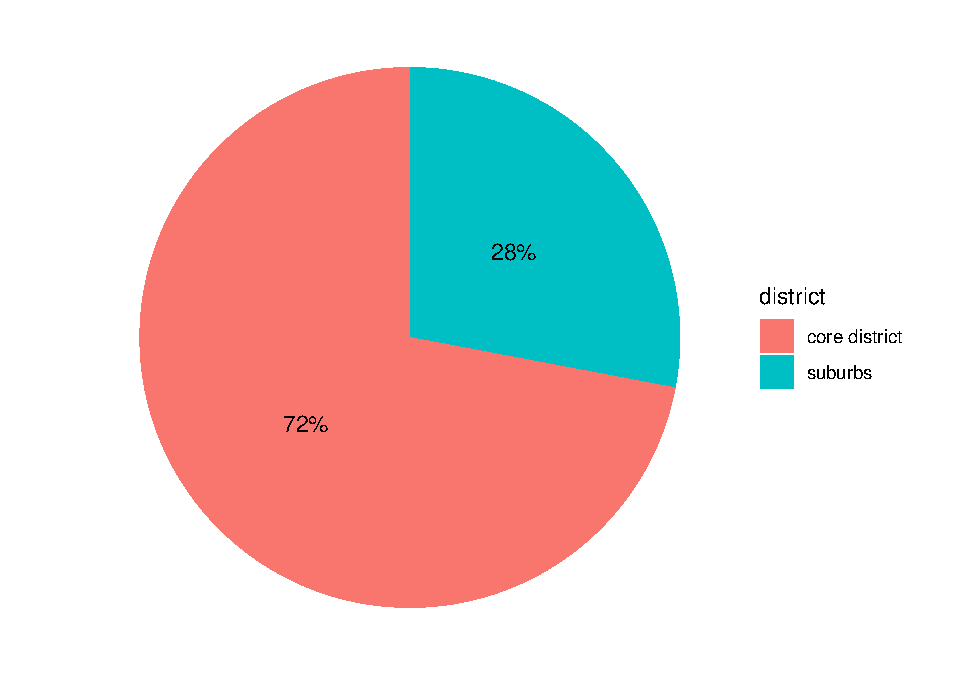
\includegraphics{Project_files/figure-latex/unnamed-chunk-22-1.pdf}

\begin{Shaded}
\begin{Highlighting}[]
\NormalTok{district\_percentage }\OtherTok{\textless{}{-}}\NormalTok{ data2017 }\SpecialCharTok{\%\textgreater{}\%}
  \FunctionTok{group\_by}\NormalTok{(district) }\SpecialCharTok{\%\textgreater{}\%}
  \FunctionTok{count}\NormalTok{(district) }\SpecialCharTok{\%\textgreater{}\%}
  \FunctionTok{mutate}\NormalTok{(}\AttributeTok{percentage=}\NormalTok{n}\SpecialCharTok{*}\DecValTok{100}\SpecialCharTok{/}\DecValTok{42004}\NormalTok{) }\SpecialCharTok{\%\textgreater{}\%} \CommentTok{\# what percentage of sold houses are in each district}
  \FunctionTok{arrange}\NormalTok{(}\FunctionTok{desc}\NormalTok{(n))}
\NormalTok{district\_percentage}
\end{Highlighting}
\end{Shaded}

\begin{verbatim}
## # A tibble: 13 x 3
## # Groups:   district [13]
##    district        n percentage
##    <chr>       <int>      <dbl>
##  1 ChaoYang    14282     34.0  
##  2 ChangPing    5509     13.1  
##  3 HaiDian      4681     11.1  
##  4 FengTai      3931      9.36 
##  5 XiCheng      3777      8.99 
##  6 DongCheng    2223      5.29 
##  7 DaXing       2162      5.15 
##  8 TongZhou     1652      3.93 
##  9 ShiJingShan  1356      3.23 
## 10 ShunYi       1096      2.61 
## 11 FangShan      730      1.74 
## 12 YiZhuang      348      0.828
## 13 MenTouGou     259      0.617
\end{verbatim}

\begin{Shaded}
\begin{Highlighting}[]
\FunctionTok{table}\NormalTok{(data2017}\SpecialCharTok{$}\NormalTok{district)}\SpecialCharTok{/}\FunctionTok{length}\NormalTok{(data2017}\SpecialCharTok{$}\NormalTok{district)}\SpecialCharTok{*}\DecValTok{100}
\end{Highlighting}
\end{Shaded}

\begin{verbatim}
## 
##   ChangPing    ChaoYang      DaXing   DongCheng    FangShan     FengTai 
##  13.1147931  33.9999048   5.1468838   5.2921011   1.7378470   9.3581869 
##     HaiDian   MenTouGou ShiJingShan      ShunYi    TongZhou     XiCheng 
##  11.1436461   0.6165786   3.2281103   2.6091511   3.9327715   8.9915726 
##    YiZhuang 
##   0.8284531
\end{verbatim}

\begin{Shaded}
\begin{Highlighting}[]
\FunctionTok{table}\NormalTok{(data2017}\SpecialCharTok{$}\NormalTok{district)}
\end{Highlighting}
\end{Shaded}

\begin{verbatim}
## 
##   ChangPing    ChaoYang      DaXing   DongCheng    FangShan     FengTai 
##        5509       14282        2162        2223         730        3931 
##     HaiDian   MenTouGou ShiJingShan      ShunYi    TongZhou     XiCheng 
##        4681         259        1356        1096        1652        3777 
##    YiZhuang 
##         348
\end{verbatim}

\hypertarget{kitchen}{%
\subsubsection{3.1.13 kitchen}\label{kitchen}}

\begin{Shaded}
\begin{Highlighting}[]
\NormalTok{data2017 }\SpecialCharTok{\%\textgreater{}\%} 
  \FunctionTok{filter}\NormalTok{(kitchen }\SpecialCharTok{\textgreater{}} \DecValTok{2}\NormalTok{) }
\end{Highlighting}
\end{Shaded}

\begin{verbatim}
##             id DOM followers totalPrice price square bedRoom livingRoom kitchen
## 1 101101782929  69        78        735 26750 274.77       4          2       3
##   bathRoom constructionTime renovationCondition buildingStructure ladderRatio
## 1        2             2001                   4                 6         0.5
##   elevator fiveYearsProperty subway  district     month day totalFloor
## 1        1                 1      1 ChangPing September  13         13
##   floorRange
## 1       high
\end{verbatim}

There are two houses with more than 2 kitchens, which seem odd. Taking a
closer look, both of these houses had less than 300 square meters, which
is impossible to have 3 kitchens in fairly medium house size. Therefore,
we removed these two outliers.

\begin{Shaded}
\begin{Highlighting}[]
\NormalTok{data2017 }\OtherTok{\textless{}{-}}\NormalTok{ data2017 }\SpecialCharTok{\%\textgreater{}\%}
  \FunctionTok{filter}\NormalTok{(kitchen }\SpecialCharTok{\textless{}} \DecValTok{3}\NormalTok{)}
\end{Highlighting}
\end{Shaded}

The distribution for the number of kitchens shows that most listings
have only one kitchen in their property. However, having no kitchen is
evidently more common than having 2 kitchens in a property.

\begin{Shaded}
\begin{Highlighting}[]
\FunctionTok{ggplot}\NormalTok{(data2017, }\FunctionTok{aes}\NormalTok{(}\AttributeTok{x =}\NormalTok{ kitchen)) }\SpecialCharTok{+}
  \FunctionTok{geom\_bar}\NormalTok{(}\AttributeTok{fill =} \StringTok{"lightblue"}\NormalTok{) }\SpecialCharTok{+}
  \FunctionTok{ggtitle}\NormalTok{(}\StringTok{"Kitchen Summary"}\NormalTok{) }\SpecialCharTok{+}
  \FunctionTok{xlab}\NormalTok{(}\StringTok{"Number of Kitchens"}\NormalTok{) }\SpecialCharTok{+}
  \FunctionTok{ylab}\NormalTok{(}\StringTok{"Count"}\NormalTok{)}
\end{Highlighting}
\end{Shaded}

\includegraphics{Project_files/figure-latex/unnamed-chunk-25-1.pdf}

\hypertarget{bathroom}{%
\subsubsection{3.1.14 bathroom}\label{bathroom}}

The distribution for the number of bathrooms shows that most listings
have only one bathroom in their property. This distribution skews
heavily to the right and the count decreases as number of bathrooms
increases.

\begin{Shaded}
\begin{Highlighting}[]
\FunctionTok{ggplot}\NormalTok{(data2017, }\FunctionTok{aes}\NormalTok{(}\AttributeTok{x =}\NormalTok{ bathRoom)) }\SpecialCharTok{+}
  \FunctionTok{geom\_bar}\NormalTok{(}\AttributeTok{fill =} \StringTok{"lightblue"}\NormalTok{) }\SpecialCharTok{+}
  \FunctionTok{ggtitle}\NormalTok{(}\StringTok{"Bathroom Summary"}\NormalTok{) }\SpecialCharTok{+}
  \FunctionTok{xlab}\NormalTok{(}\StringTok{"Number of Bathrooms"}\NormalTok{) }\SpecialCharTok{+}
  \FunctionTok{ylab}\NormalTok{(}\StringTok{"Count"}\NormalTok{)}
\end{Highlighting}
\end{Shaded}

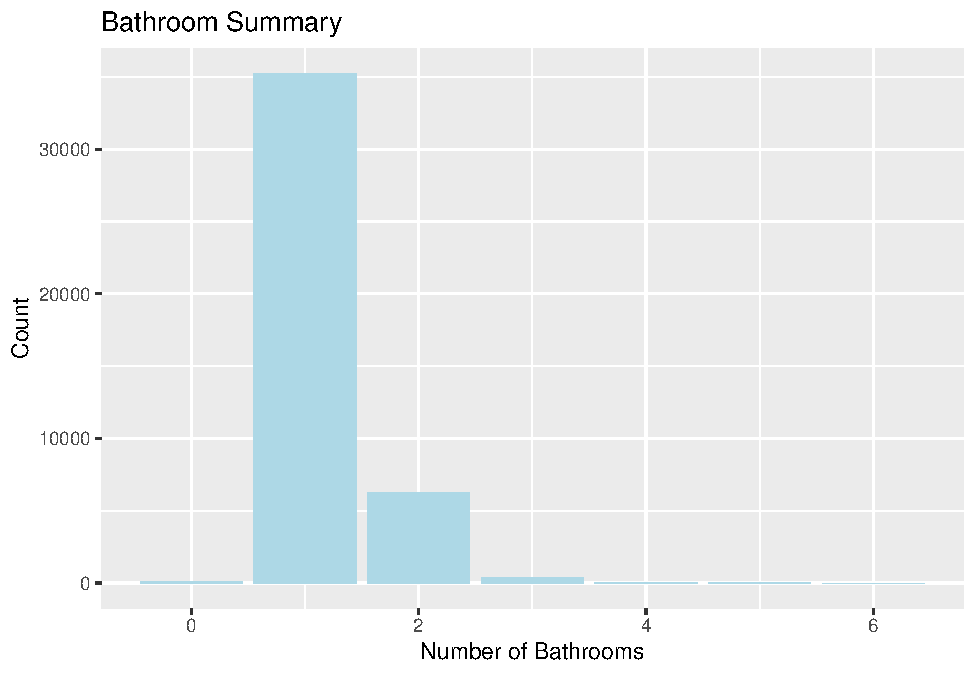
\includegraphics{Project_files/figure-latex/unnamed-chunk-26-1.pdf}

\hypertarget{construction-time}{%
\subsubsection{3.1.15 construction time}\label{construction-time}}

\begin{Shaded}
\begin{Highlighting}[]
\FunctionTok{table}\NormalTok{(data2017}\SpecialCharTok{$}\NormalTok{constructionTime)}
\end{Highlighting}
\end{Shaded}

\begin{verbatim}
## 
## 1950 1952 1953 1954 1955 1956 1957 1958 1959 1960 1961 1962 1963 1964 1965 1966 
##    1    1    2    9    6    9   10   21   13   31    2    5   16   23   35   22 
## 1967 1968 1969 1970 1971 1972 1973 1974 1975 1976 1977 1978 1979 1980 1981 1982 
##    6    2    1   63    2    5   22   30   49   68   66  130  224  547  330  396 
## 1983 1984 1985 1986 1987 1988 1989 1990 1991 1992 1993 1994 1995 1996 1997 1998 
##  424  488  640  679  736  790  778 1151  647 1162  965 1142 1217 1215  911 1371 
## 1999 2000 2001 2002 2003 2004 2005 2006 2007 2008 2009 2010 2011 2012 2013 2014 
## 1276 1801 1351 1497 2284 2525 2425 1888 1780 1740 1798 1430 1000 1043  626  781 
## 2015 2016 
##  259   38
\end{verbatim}

\begin{Shaded}
\begin{Highlighting}[]
\FunctionTok{median}\NormalTok{(data2017}\SpecialCharTok{$}\NormalTok{constructionTime)}
\end{Highlighting}
\end{Shaded}

\begin{verbatim}
## [1] 2002
\end{verbatim}

\begin{Shaded}
\begin{Highlighting}[]
\FunctionTok{mean}\NormalTok{(data2017}\SpecialCharTok{$}\NormalTok{constructionTime)}
\end{Highlighting}
\end{Shaded}

\begin{verbatim}
## [1] 1999.547
\end{verbatim}

The year of construction of the listings that were transacted in 2017
ranges from the year 1950 to the year 2016. Out of all the included
listings, most of the properties were built in the year 2004
accumulating a total of 2525 properties.

The distribution skews to the left as the median of the year 2002 and
mean of the year 1999 both lie to the left of the mode of the year 2004.

\begin{Shaded}
\begin{Highlighting}[]
\FunctionTok{ggplot}\NormalTok{(data2017, }\FunctionTok{aes}\NormalTok{(}\AttributeTok{x =}\NormalTok{ constructionTime)) }\SpecialCharTok{+}
  \FunctionTok{geom\_bar}\NormalTok{(}\AttributeTok{fill =} \StringTok{"lightblue"}\NormalTok{) }\SpecialCharTok{+}
  \FunctionTok{ggtitle}\NormalTok{(}\StringTok{"Time of Construction Summary"}\NormalTok{) }\SpecialCharTok{+}
  \FunctionTok{xlab}\NormalTok{(}\StringTok{"Time of Construction"}\NormalTok{) }\SpecialCharTok{+}
  \FunctionTok{ylab}\NormalTok{(}\StringTok{"Count"}\NormalTok{)}
\end{Highlighting}
\end{Shaded}

\includegraphics{Project_files/figure-latex/unnamed-chunk-29-1.pdf}

\hypertarget{renovation-condition}{%
\subsubsection{3.1.16 renovation condition}\label{renovation-condition}}

The condition of renovation

The distribution for the condition of renovation shows that most
listings have the highest score of 4 in terms of the condition of
renovation for their listing. This distribution skews heavily to the
left.

\begin{Shaded}
\begin{Highlighting}[]
\FunctionTok{ggplot}\NormalTok{(data2017, }\FunctionTok{aes}\NormalTok{(}\AttributeTok{x =}\NormalTok{ renovationCondition)) }\SpecialCharTok{+}
  \FunctionTok{geom\_bar}\NormalTok{(}\AttributeTok{fill =} \StringTok{"lightblue"}\NormalTok{) }\SpecialCharTok{+}
  \FunctionTok{ggtitle}\NormalTok{(}\StringTok{"Condition of Renovation Summary"}\NormalTok{) }\SpecialCharTok{+}
  \FunctionTok{xlab}\NormalTok{(}\StringTok{"Condition of Renovation"}\NormalTok{) }\SpecialCharTok{+}
  \FunctionTok{ylab}\NormalTok{(}\StringTok{"Count"}\NormalTok{)}
\end{Highlighting}
\end{Shaded}

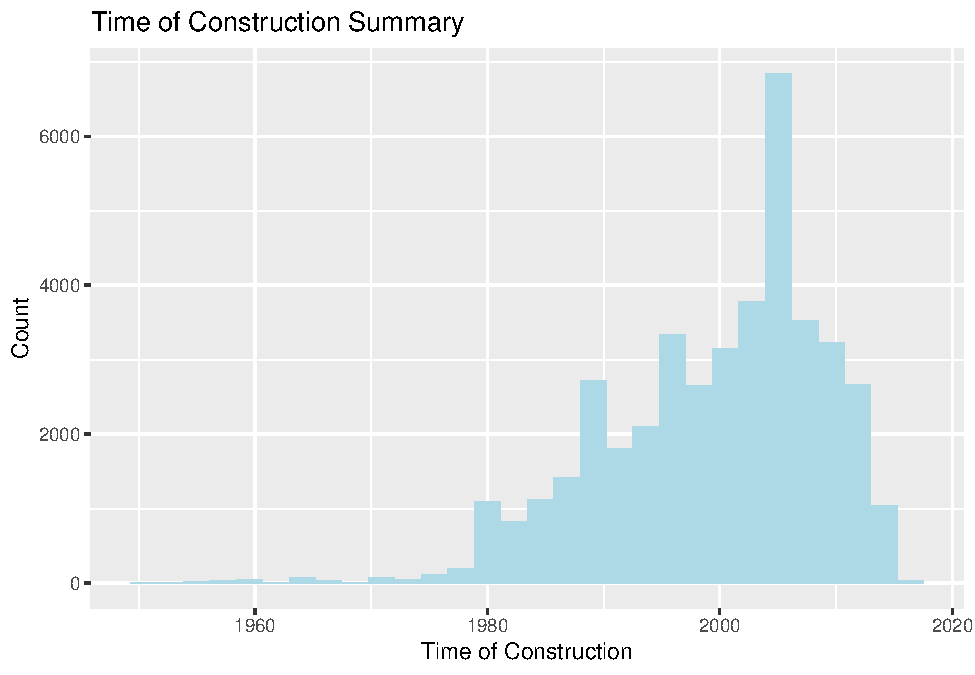
\includegraphics{Project_files/figure-latex/unnamed-chunk-30-1.pdf}

\hypertarget{building-structure}{%
\subsubsection{3.1.17 building structure}\label{building-structure}}

The distribution for the building structure shows that most listings are
made of steel-concrete composite. This distribution skews heavily to the
left.

\begin{Shaded}
\begin{Highlighting}[]
\FunctionTok{ggplot}\NormalTok{(data2017, }\FunctionTok{aes}\NormalTok{(}\AttributeTok{x =}\NormalTok{ buildingStructure)) }\SpecialCharTok{+}
  \FunctionTok{geom\_bar}\NormalTok{(}\AttributeTok{fill =} \StringTok{"lightblue"}\NormalTok{) }\SpecialCharTok{+}
  \FunctionTok{ggtitle}\NormalTok{(}\StringTok{"Structure of Building Summary"}\NormalTok{) }\SpecialCharTok{+}
  \FunctionTok{xlab}\NormalTok{(}\StringTok{"Structure of Building"}\NormalTok{) }\SpecialCharTok{+}
  \FunctionTok{ylab}\NormalTok{(}\StringTok{"Count"}\NormalTok{)}
\end{Highlighting}
\end{Shaded}

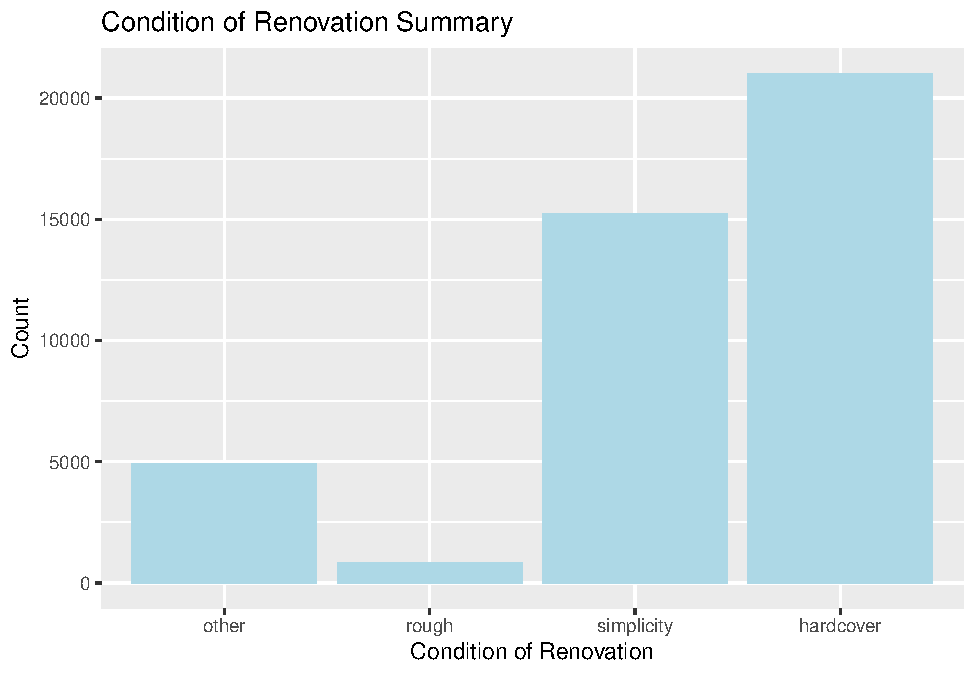
\includegraphics{Project_files/figure-latex/unnamed-chunk-31-1.pdf}

\hypertarget{ladder-ratio}{%
\subsubsection{3.1.18 ladder ratio}\label{ladder-ratio}}

The maximum value for ladderRatio is 10009400, which seems like a typo,
so we decided to remove this observation.

\begin{Shaded}
\begin{Highlighting}[]
\NormalTok{data2017 }\OtherTok{\textless{}{-}}\NormalTok{ data2017 }\SpecialCharTok{\%\textgreater{}\%} 
  \FunctionTok{filter}\NormalTok{(ladderRatio }\SpecialCharTok{\textless{}} \DecValTok{5}\NormalTok{)}
\end{Highlighting}
\end{Shaded}

\begin{Shaded}
\begin{Highlighting}[]
\FunctionTok{table}\NormalTok{(data2017}\SpecialCharTok{$}\NormalTok{ladderRatio)}
\end{Highlighting}
\end{Shaded}

\begin{verbatim}
## 
## 0.014 0.015  0.02 0.022 0.023 0.025 0.026 0.028 0.029  0.03 0.031 0.033 0.034 
##    10     2    18     3     2     1     2     9     3     2     6    12     1 
## 0.035 0.036 0.037 0.038 0.039  0.04 0.041 0.042 0.043 0.045 0.047 0.048  0.05 
##     2     8     1    12     3     6     1    11     4     7     5     8    18 
## 0.053 0.054 0.056 0.057 0.059  0.06 0.061 0.062 0.065 0.067 0.069 0.071 0.074 
##     9     8    11    15    64     1    13    19     6    14     4    24     5 
## 0.075 0.077  0.08 0.081 0.083 0.086 0.087 0.088 0.091 0.095 0.098   0.1 0.103 
##     1    35     9     9    42    20    39     1    46    14    16   109    38 
## 0.105 0.107 0.108 0.111 0.114 0.118  0.12 0.121 0.125 0.129  0.13 0.133 0.136 
##    31    11     6   191     1    42    29    18   406    10    31    37    25 
## 0.138 0.143 0.148  0.15 0.154 0.156 0.158  0.16 0.161 0.162 0.167 0.171 0.174 
##    19   377    16    26   128     1    31     7    12    13   929     5    62 
## 0.176 0.179 0.182 0.185 0.188 0.189  0.19 0.192 0.198   0.2 0.208 0.211 0.214 
##    40     2   204     1    66     1    41    19     3  1842     2    59   182 
## 0.217 0.222 0.227 0.231 0.235 0.238  0.24  0.25 0.255 0.261 0.263 0.267 0.273 
##    11   514    15   124    45     1     2  5735     1    11    21    14   221 
## 0.276 0.278 0.286   0.3 0.304 0.308 0.312 0.318 0.333 0.345 0.346 0.353 0.364 
##     2     9   963   847    13     5     3     2  9242     9     7     1    37 
##  0.37 0.375 0.385   0.4 0.417 0.429 0.438 0.444 0.467   0.5 0.538 0.571 0.583 
##    12   618    16  1009     1    76     2    56     1 14602     2     6     2 
##   0.6 0.625 0.667 0.714  0.75   0.8 0.818 0.833  0.87 0.889     1  1.25 1.333 
##    18     7  1184     1    45     3     1     2     3     3   724     2    21 
##   1.5 1.667     2     3 
##    54     1    21     1
\end{verbatim}

\begin{Shaded}
\begin{Highlighting}[]
\FunctionTok{median}\NormalTok{(data2017}\SpecialCharTok{$}\NormalTok{ladderRatio)}
\end{Highlighting}
\end{Shaded}

\begin{verbatim}
## [1] 0.333
\end{verbatim}

\begin{Shaded}
\begin{Highlighting}[]
\FunctionTok{mean}\NormalTok{(data2017}\SpecialCharTok{$}\NormalTok{ladderRatio)}
\end{Highlighting}
\end{Shaded}

\begin{verbatim}
## [1] 0.3797018
\end{verbatim}

The distribution for the ladder ratio shows that most listings have 2
residents to one elevator per floor. This distribution skews heavily to
the left as the average number of residents sharing an elevator per
floor is 3.

\begin{Shaded}
\begin{Highlighting}[]
\FunctionTok{ggplot}\NormalTok{(data2017, }\FunctionTok{aes}\NormalTok{(}\AttributeTok{x =}\NormalTok{ ladderRatio)) }\SpecialCharTok{+}
  \FunctionTok{geom\_bar}\NormalTok{(}\AttributeTok{fill =} \StringTok{"lightblue"}\NormalTok{, }\AttributeTok{width =} \FloatTok{0.05}\NormalTok{) }\SpecialCharTok{+}
  \FunctionTok{ggtitle}\NormalTok{(}\StringTok{"Ladder Ratio Summary"}\NormalTok{) }\SpecialCharTok{+}
  \FunctionTok{xlab}\NormalTok{(}\StringTok{"Ladder Ratio"}\NormalTok{) }\SpecialCharTok{+}
  \FunctionTok{ylab}\NormalTok{(}\StringTok{"Count"}\NormalTok{)}
\end{Highlighting}
\end{Shaded}

\begin{verbatim}
## Warning: position_stack requires non-overlapping x intervals
\end{verbatim}

\includegraphics{Project_files/figure-latex/unnamed-chunk-35-1.pdf}

\hypertarget{elevator}{%
\subsubsection{3.1.19 elevator}\label{elevator}}

The distribution for the presence of an elevator shows that it is more
common for listings to have at lease one elevator in the building
compared to none at all.

\begin{Shaded}
\begin{Highlighting}[]
\FunctionTok{ggplot}\NormalTok{(data2017, }\FunctionTok{aes}\NormalTok{(}\AttributeTok{x =}\NormalTok{ elevator)) }\SpecialCharTok{+}
  \FunctionTok{geom\_bar}\NormalTok{(}\AttributeTok{fill =} \StringTok{"lightblue"}\NormalTok{) }\SpecialCharTok{+}
  \FunctionTok{ggtitle}\NormalTok{(}\StringTok{"Availability of Elevator"}\NormalTok{) }\SpecialCharTok{+}
  \FunctionTok{xlab}\NormalTok{(}\StringTok{"Elevator"}\NormalTok{) }\SpecialCharTok{+}
  \FunctionTok{ylab}\NormalTok{(}\StringTok{"Count"}\NormalTok{)}
\end{Highlighting}
\end{Shaded}

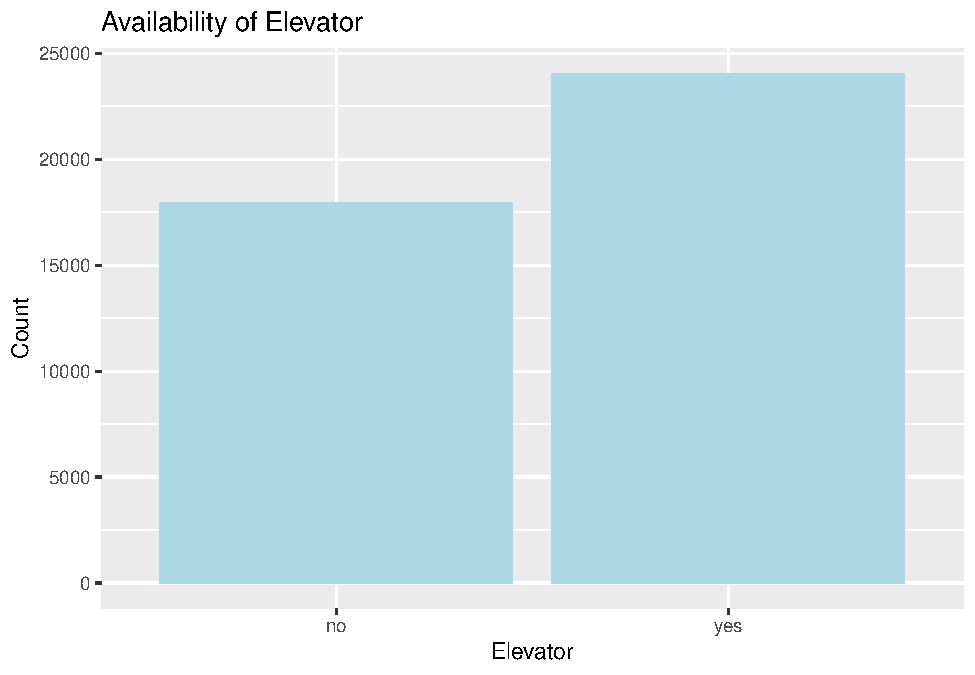
\includegraphics{Project_files/figure-latex/unnamed-chunk-36-1.pdf}

\hypertarget{five-years-property}{%
\subsubsection{3.1.20 five years property}\label{five-years-property}}

The distribution for whether the previous has stayed in the listing for
less than five years shows that most sellers stay in their property for
less than five years.

\begin{Shaded}
\begin{Highlighting}[]
\FunctionTok{ggplot}\NormalTok{(data2017, }\FunctionTok{aes}\NormalTok{(}\AttributeTok{x =}\NormalTok{ fiveYearsProperty)) }\SpecialCharTok{+}
  \FunctionTok{geom\_bar}\NormalTok{(}\AttributeTok{fill =} \StringTok{"lightblue"}\NormalTok{) }\SpecialCharTok{+}
  \FunctionTok{ggtitle}\NormalTok{(}\StringTok{"Five Years Property Summary"}\NormalTok{) }\SpecialCharTok{+}
  \FunctionTok{xlab}\NormalTok{(}\StringTok{"Five Years Property"}\NormalTok{) }\SpecialCharTok{+}
  \FunctionTok{ylab}\NormalTok{(}\StringTok{"Count"}\NormalTok{)}
\end{Highlighting}
\end{Shaded}

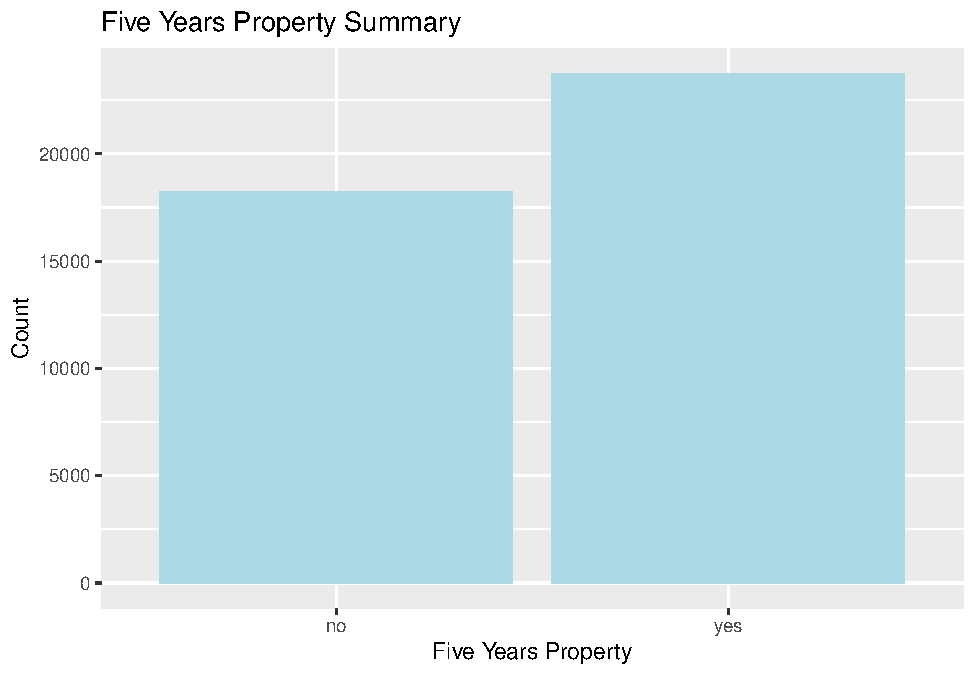
\includegraphics{Project_files/figure-latex/unnamed-chunk-37-1.pdf}

\hypertarget{subway}{%
\subsubsection{3.1.21 subway}\label{subway}}

The distribution for the presence of any nearby subways shows that it is
more common for listings to have at lease one subway nearby the building
compared to none at all.

\begin{Shaded}
\begin{Highlighting}[]
\FunctionTok{ggplot}\NormalTok{(data2017, }\FunctionTok{aes}\NormalTok{(}\AttributeTok{x =}\NormalTok{ subway)) }\SpecialCharTok{+}
  \FunctionTok{geom\_bar}\NormalTok{(}\AttributeTok{fill =} \StringTok{"lightblue"}\NormalTok{) }\SpecialCharTok{+}
  \FunctionTok{ggtitle}\NormalTok{(}\StringTok{"Subway Summary"}\NormalTok{) }\SpecialCharTok{+}
  \FunctionTok{xlab}\NormalTok{(}\StringTok{"Availability of Nearby Subways"}\NormalTok{) }\SpecialCharTok{+}
  \FunctionTok{ylab}\NormalTok{(}\StringTok{"Count"}\NormalTok{)}
\end{Highlighting}
\end{Shaded}

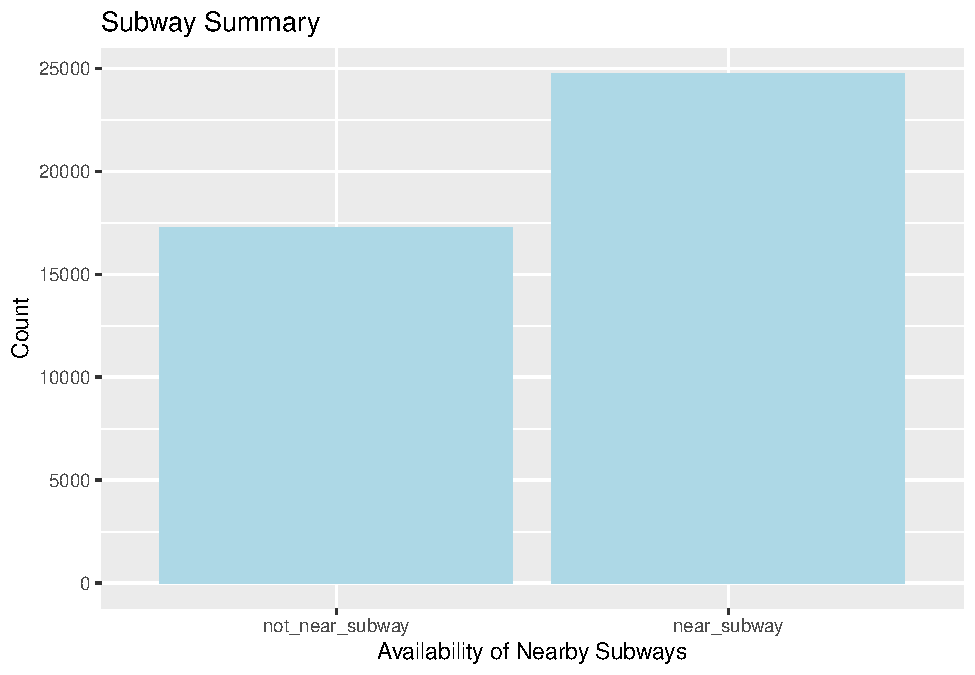
\includegraphics{Project_files/figure-latex/unnamed-chunk-38-1.pdf}

\hypertarget{relationships-between-variables}{%
\subsection{3.2 Relationships between
variables}\label{relationships-between-variables}}

\hypertarget{price-vs.-district}{%
\subsubsection{3.2.1 price vs.~district}\label{price-vs.-district}}

\hypertarget{price-vs.-dom}{%
\subsubsection{3.2.2 price vs.~DOM}\label{price-vs.-dom}}

\hypertarget{price-vs.-construction-time}{%
\subsubsection{3.2.3 price vs.~construction
time}\label{price-vs.-construction-time}}

\hypertarget{construction-time-vs.-renovation-condition}{%
\subsubsection{3.2.4 construction time vs.~renovation
condition}\label{construction-time-vs.-renovation-condition}}

\hypertarget{construction-time-vs.-building-structure}{%
\subsubsection{3.2.5 construction time vs.~building
structure}\label{construction-time-vs.-building-structure}}

\hypertarget{work-cited}{%
\subsubsection{\texorpdfstring{\textbf{Work
Cited}}{Work Cited}}\label{work-cited}}

\hypertarget{some-online-resources-that-i-think-might-be-helpful}{%
\subsection{some online resources that I think might be
helpful}\label{some-online-resources-that-i-think-might-be-helpful}}

\begin{enumerate}
\def\labelenumi{\arabic{enumi}.}
\tightlist
\item
  It mentions the price drop on beijing houses in 2017 because of some
  regulations
  \url{http://www.xinhuanet.com/english/2018-01/29/c_136933533.htm}
\end{enumerate}

\hypertarget{model}{%
\section{4 Model}\label{model}}

\hypertarget{split-data-into-train-and-test}{%
\subsection{4.1 Split data into train and
test}\label{split-data-into-train-and-test}}

\begin{Shaded}
\begin{Highlighting}[]
\FunctionTok{set.seed}\NormalTok{(}\DecValTok{428}\NormalTok{)}
\NormalTok{index }\OtherTok{\textless{}{-}} \FunctionTok{sample}\NormalTok{(}\FunctionTok{nrow}\NormalTok{(data2017),}\DecValTok{21002}\NormalTok{,}\AttributeTok{replace =} \ConstantTok{FALSE}\NormalTok{)}
\NormalTok{train }\OtherTok{\textless{}{-}}\NormalTok{ data2017[index,}\FunctionTok{c}\NormalTok{(}\DecValTok{2}\NormalTok{,}\DecValTok{3}\NormalTok{,}\DecValTok{5}\SpecialCharTok{:}\DecValTok{22}\NormalTok{)] }\CommentTok{\# exclude total price }
\NormalTok{test }\OtherTok{\textless{}{-}}\NormalTok{ data2017[}\SpecialCharTok{{-}}\NormalTok{index,}\FunctionTok{c}\NormalTok{(}\DecValTok{2}\NormalTok{,}\DecValTok{3}\NormalTok{,}\DecValTok{5}\SpecialCharTok{:}\DecValTok{22}\NormalTok{)] }\CommentTok{\# exclude total price}
\end{Highlighting}
\end{Shaded}

I splited the data in half, into train and test data. Train data is used
to train the model, while test data is used to test the accuracy of
prediction from the model.

\hypertarget{linear-model}{%
\subsection{4.2 Linear Model}\label{linear-model}}

\begin{Shaded}
\begin{Highlighting}[]
\NormalTok{linear\_model }\OtherTok{\textless{}{-}} \FunctionTok{lm}\NormalTok{(price}\SpecialCharTok{\textasciitilde{}}\NormalTok{., }\AttributeTok{data =}\NormalTok{ train)}
\FunctionTok{summary}\NormalTok{(linear\_model)}
\end{Highlighting}
\end{Shaded}

\begin{verbatim}
## 
## Call:
## lm(formula = price ~ ., data = train)
## 
## Residuals:
##    Min     1Q Median     3Q    Max 
## -90243  -8035   -728   7114  77498 
## 
## Coefficients:
##                       Estimate Std. Error t value Pr(>|t|)    
## (Intercept)         319394.764  29876.587  10.690  < 2e-16 ***
## DOM                     13.529      1.889   7.161 8.30e-13 ***
## followers              -39.908      1.705 -23.407  < 2e-16 ***
## square                -178.423      5.671 -31.463  < 2e-16 ***
## bedRoom               1291.276    194.308   6.645 3.10e-11 ***
## livingRoom            1742.334    254.948   6.834 8.48e-12 ***
## kitchen              10231.539   1026.962   9.963  < 2e-16 ***
## bathRoom              6004.744    329.839  18.205  < 2e-16 ***
## constructionTime      -141.801     14.975  -9.469  < 2e-16 ***
## renovationCondition   1014.437     98.944  10.253  < 2e-16 ***
## buildingStructure      395.000     91.385   4.322 1.55e-05 ***
## ladderRatio          11872.746    636.657  18.649  < 2e-16 ***
## elevator1             5187.584    382.891  13.548  < 2e-16 ***
## fiveYearsProperty1    -210.859    196.589  -1.073 0.283468    
## subway1               5321.838    206.239  25.804  < 2e-16 ***
## districtChaoYang     17042.019    335.527  50.792  < 2e-16 ***
## districtDaXing         352.731    493.000   0.715 0.474321    
## districtDongCheng    46435.489    522.019  88.954  < 2e-16 ***
## districtFangShan     -9717.909    793.713 -12.244  < 2e-16 ***
## districtFengTai       9927.710    420.564  23.606  < 2e-16 ***
## districtHaiDian      35387.219    399.079  88.672  < 2e-16 ***
## districtMenTouGou    -2678.271   1184.017  -2.262 0.023706 *  
## districtShiJingShan   7886.015    600.493  13.133  < 2e-16 ***
## districtShunYi       -4983.484    638.082  -7.810 5.98e-15 ***
## districtTongZhou      1576.939    539.824   2.921 0.003490 ** 
## districtXiCheng      55756.138    440.600 126.546  < 2e-16 ***
## districtYiZhuang     -2420.212   1035.994  -2.336 0.019494 *  
## monthAugust          -8000.127    571.492 -13.999  < 2e-16 ***
## monthDecember       -10608.009    533.145 -19.897  < 2e-16 ***
## monthFebruary        -5435.901    482.284 -11.271  < 2e-16 ***
## monthJanuary         -8174.648    516.729 -15.820  < 2e-16 ***
## monthJuly            -6399.466    580.502 -11.024  < 2e-16 ***
## monthJune            -5247.642    633.098  -8.289  < 2e-16 ***
## monthMarch           -1135.593    472.512  -2.403 0.016256 *  
## monthMay             -1642.461    652.030  -2.519 0.011776 *  
## monthNovember        -9879.886    552.689 -17.876  < 2e-16 ***
## monthOctober        -10153.341    566.487 -17.923  < 2e-16 ***
## monthSeptember       -8204.059    544.111 -15.078  < 2e-16 ***
## day                      4.974     11.819   0.421 0.673870    
## totalFloor             -94.303     19.403  -4.860 1.18e-06 ***
## floorRangehigh       -1128.214    394.266  -2.862 0.004220 ** 
## floorRangelow        -1427.983    398.370  -3.585 0.000338 ***
## floorRangemidium      -527.733    366.660  -1.439 0.150080    
## floorRangetop        -2930.316    436.780  -6.709 2.01e-11 ***
## ---
## Signif. codes:  0 '***' 0.001 '**' 0.01 '*' 0.05 '.' 0.1 ' ' 1
## 
## Residual standard error: 13490 on 20958 degrees of freedom
## Multiple R-squared:  0.6886, Adjusted R-squared:  0.6879 
## F-statistic:  1078 on 43 and 20958 DF,  p-value: < 2.2e-16
\end{verbatim}

Based on the results of linear model, all the variables are important
except for five year property and the day of month being sold.

\begin{Shaded}
\begin{Highlighting}[]
\CommentTok{\# training MSE}
\NormalTok{pred\_train\_lm }\OtherTok{\textless{}{-}} \FunctionTok{predict}\NormalTok{(linear\_model, train, }\AttributeTok{type=}\StringTok{"response"}\NormalTok{)}
\FunctionTok{mean}\NormalTok{((pred\_train\_lm}\SpecialCharTok{{-}}\NormalTok{train}\SpecialCharTok{$}\NormalTok{price)}\SpecialCharTok{\^{}}\DecValTok{2}\NormalTok{)}
\end{Highlighting}
\end{Shaded}

\begin{verbatim}
## [1] 181660789
\end{verbatim}

\begin{Shaded}
\begin{Highlighting}[]
\CommentTok{\# testing MSE}
\NormalTok{pred\_test\_lm }\OtherTok{\textless{}{-}} \FunctionTok{predict}\NormalTok{(linear\_model, test, }\AttributeTok{type=}\StringTok{"response"}\NormalTok{)}
\FunctionTok{mean}\NormalTok{((pred\_test\_lm}\SpecialCharTok{{-}}\NormalTok{test}\SpecialCharTok{$}\NormalTok{price)}\SpecialCharTok{\^{}}\DecValTok{2}\NormalTok{)}
\end{Highlighting}
\end{Shaded}

\begin{verbatim}
## [1] 178229364
\end{verbatim}

For now, the MSE looks pretty big. Let's take a look at other models.

\hypertarget{random-forest}{%
\subsection{4.2 Random Forest}\label{random-forest}}

\end{document}
